%Update 9/7/2022
\documentclass{article}     %type of document
\usepackage[utf8]{inputenc} %for text encoding
\usepackage{../lambdatex} 
\everymath{\displaystyle}

\title{Funzioni reali di variabili reali}
\author{Davide Borra - 5LA}
\date{A.S. 2021-2022}

\begin{document}
    \begin{titlepage}
    \maketitle
    \tableofcontents
    \vspace{\fill}
    \hspace{\fill} v. 1.2   %incrementare primo numero per contenuti e secondo numero per patch
    \end{titlepage}
    
    \lhead{Funzioni reali di variabili reali}
    \chead{}
    \rhead{Davide Borra - 5LA}

    \section{Definizione e caratteristiche}
        \begin{definition}
            Presi due insiemi $D$ (dominio) e $C$ (codominio) tali che $D \subset \R$ e $C \subset \R$, si dice \textbf{funzione} $f$ da $D$ a $C$ una relazione che ad ogni elemento di $D$ associa uno e un solo elemento di $D$. In simboli \[f:D\rightarrow C\]
        \end{definition}
        Se ad ogni elemento $x \in D$ la funzione $f$ associa un elemento $y\in C$, $y$ (\textbf{variabile dipendente}) è detta \textbf{immagine} di $x$, mentre $x$ (\textbf{variabile indipendente}) è detta \textbf{controimmagine} di $y$. La scrittura $y=f(x)$ è detta \textbf{espressione analitica della funzione in forma esplicita}. Le funzioni possono anche essere scritte in forma implicita come $g(x,y)=0$
    
    \subsection{Classificazione}
        Le funzioni si dividono in due grandi categorie: le funzioni algebriche e le funzioni trascendenti. Una funzione si dice \textbf{algebrica} se la sua espressione analitica contiene solo operazioni di somma algebrica, moltiplicazione, divisione, elevamento a potenza ed estrazione di radice, altrimenti si dice \textbf{trascendente}. Le funzioni algebriche sono a loro volta divise in \begin{itemize}
            \item \textbf{funzioni polinomiali}: possono essere scritte sotto forma di polinomi. Esse sono dette \textit{lineari} se il polinomio che le identifica è di primo grado rispetto alla variabile indipendente, \textit{quadratiche} se è di secondo grado e \textit{cubiche} se di terzo.
            \item \textbf{funzioni fratte}: possono essere scritte come quoziente di due polinomi, o comunque la loro scrittura analitica presenta una variabile $x$ al denominatore.
            \item \textbf{funzioni irrazionali}: nella scrittura analitica conmpare un radicale al cui radicando è presente la variabile $x$.
        \end{itemize}
    \subsection{Dominio}
        \begin{definition}
            Si dice \textbf{dominio naturale} o \textbf{campo di esistenza} di una funzione $y=f(x)$ l'insieme più ampio dei valori reali che è ossibile assegnare alla variabile $x$ per far sì che esista anche il corrispondente valore i $y$
        \end{definition}

        \begin{longtable}[h]{| p{0.45\textwidth} | p{0.45\textwidth }|}
            \hline
            Funzione & Dominio \\ \hline \hline \endhead
            \raisebox{8pt}{\phantom{M}} Funzioni polinomiali & \\
            \[y=a_n x^n+a_{n-1}x^{n-1}+\dots+a_1x^1+a_0\] & \[\R\]\\ \hline
            \raisebox{8pt}{\phantom{M}} Funzioni fratte &\\
            \[y=\frac{P(x)}{Q(x)}~~~P \text{ e } Q\text{ polinomi}\] & \[\R - \{x\in\R|Q(x)=0\}\]\\ \hline
            \raisebox{8pt}{\phantom{M}} Funzioni irrazionali &\\
            \[y=\sqrt[n]{f(x)}\] & \[\langle \begin{array}{l}
                \{x\in \R|f(x)\geq 0 \}\text{ se } n \text{ pari}\\
                \text{dominio di } f(x) \text{ se } n \text{ dispari}
            \end{array}\]\\ \hline
            \raisebox{8pt}{\phantom{M}} Funzioni logaritmiche &\\
            \[y=\log_a f(x)\text{~~~con } a>0 \land a\neq 1\] & \[\{x\in \R|f(x)>0\}\] \\ \hline
            \raisebox{8pt}{\phantom{M}} Funzioni esponenziali &\\

            \[\renewcommand{\arraystretch}{1.5}\begin{array}{ll}
                y=a^{f(x)} &\text{con } a>0 \land a\neq 1\\
                y=[f(x)]^{g(x)} \\
                f(x)^\alpha & \renewcommand{\arraystretch}{1}\begin{array}{l}
                    \alpha \text{ irrazionale}\\
                    \text{se }\alpha>0\\
                    \text{se }\alpha<0
                \end{array}\\ 
            \end{array}\] &
            \[\renewcommand{\arraystretch}{1.5}\begin{array}{l}
                \text{dominio di }f(x)\\
                \{x\in\R|f(x)>0\}\cap\text{dominio di }g(x)\\
                \renewcommand{\arraystretch}{1}\begin{array}{l}
                     \\
                    f(x)\geq 0\\
                    f(x)>0
                \end{array}
            \end{array}\] \\ \hline
            \raisebox{8pt}{\phantom{M}} Funzioni goniometriche &\\
            \[
                \renewcommand{\arraystretch}{1.5}\begin{array}{l}
                    y=\sin x, y=\cos x\\
                    y=\tg x\\
                    y=\cotg x\\
                    y=\arcsin x, y=\arccos x\\
                    y=\arctg x, y=\arccotg x
                \end{array}
            \] &
            \[
                \renewcommand{\arraystretch}{1.5}\begin{array}{l}
                    \R\\
                    \R -{\frac{\pi}{2}+k\pi}\text{, con } k\in\Z\\
                    \R -{k\pi}\text{, con } k\in\Z\\
                    \left[-1,1\right]\\
                    \R
                \end{array}
            \]\\ \hline
        \end{longtable}
        
    \subsection{Zeri di funzione}
        \begin{definition}
            Preso un numero reale $\lambda$, si dice zero (radice) della funzione $y=f(x)$ se $f(\lambda)=0$
        \end{definition}
        \begin{theorem}[Teorema fondamentale dell'algebra]
            Sia $P(x)$ un polinomio di grado $n$ a coefficienti reali. Nell'insieme dei numeri reali, esso ha al più $n$ radici.
        \end{theorem}
    \subsection{Studio del segno}
        Data una funzione $y=f(x)$, essa può assumere sia valori positivi che valori negativi. Studiare il segno di una funzione significa determinare per quali intervalli di valori della variabile $x$, la variabile $y$ assume valori positivi, e per quali valori negativi. Generalmente per determinare il segno di una funzione è sufficiente risolvere la disequazione \[f(x)>0\]
        \begin{ex}
            Si determinino dominio, radici e segno della funzione $y=x^2+x-2$
        \end{ex}
            \begin{enumerate}
                \item[-] Dominio: Si tratta di una funzione polinomiale, di conseguenza il suo dominio è l'insieme $\R$
                \item[-] Zeri: Per determinare gli zeri bisogna risolvere l'equazione $f(x)=0$, ovvero \[x^2+x-2=0\]\[(x-1)(x+2)=0\]\[x_1=1~~~~x_2=-2\]
                \item[-] Segno: Risolviamo la disequazione \[x^2+x-2>0\]\[(x-1)(x+2)>0\]\[\text{prodotto di fattori } >0 \text{: soluzioni esterne }x<-2\lor x>1\]
            \end{enumerate}
    \section{Proprietà}
        \subsection{Funzioni iniettive, suriettive e biiettive}
        \begin{definition}
            Data una funzione $f:D\rightarrow C$, essa si dice:
            \begin{itemize}
                \item \textbf{iniettiva} se ogni elemento di $C$ è immagine di \textnormal{al più} un elemento di $D$
                \item \textbf{suriettiva} se ogni elemento di $C$ è immagine di \textnormal{almeno} un elemento di $D$
                \item \textbf{biiettiva} se è sia iniettiva che suriettiva.
            \end{itemize}
            Per dimostrare che una funzione è iniettiva, è possibile dimostrare che $\forall x_1,x_2 \in D, x_1\neq x_2\rightarrow f(x_1)\neq f(x_2)$.\\
            Ogni funzione è suriettiva nel proprio codominio, per questo generalmente la suriettività viene analizzata in $\R$.
        \end{definition}
        Un metodo semplice per capire dal grafico se una funzione è iniettiva e/o suriettiva (attenzione, non equivale ad una dimostrazione) è il criterio della retta orizzontale. Una funzione è iniettiva se ogni retta parallela all'asse $x$ che è possibile tracciare interseca la funzione in \textit{al più} un punto, suriettiva se la interseca in \textit{almeno} un punto e biiettiva se in \textit{esattamente} un punto.
    \subsection{Monotonia}
        \begin{definition}[Funzione crescente in senso stretto]
            Data una funzione $y=f(x)$ di dominio $D\subseteq \R$, essa si dice \textbf{crescente in senso stretto} in un intervallo $I\subseteq D$ se $\forall x_1,x_2 \in I, x_1 <x_2 \rightarrow f(x_1)<f(x_2)$.
        \end{definition}
        \begin{definition}[Funzione crescente in senso lato]
            Data una funzione $y=f(x)$ di dominio $D\subseteq \R$, essa si dice \textbf{crescente in senso lato} (o \textbf{non decrescente}) in un intervallo $I\subseteq D$ se $\forall x_1,x_2 \in I, x_1 <x_2 \rightarrow f(x_1)\leq f(x_2)$.
        \end{definition}
        \begin{definition}[Funzione decrescente in senso stretto]
            Data una funzione $y=f(x)$ di dominio $D\subseteq \R$, essa si dice \textbf{decrescente in senso stretto} in un intervallo $I\subseteq D$ se $\forall x_1,x_2 \in I, x_1 <x_2 \rightarrow f(x_1)>f(x_2)$.
        \end{definition}
        \begin{definition}[Funzione decrescente in senso lato]
            Data una funzione $y=f(x)$ di dominio $D\subseteq \R$, essa si dice \textbf{decre- scente in senso lato} (o \textbf{non crescente}) in un intervallo $I\subseteq D$ se $\forall x_1,x_2 \in I, x_1 <x_2 \rightarrow f(x_1)\geq f(x_2)$. 
        \end{definition}
        \begin{ex}
        \end{ex}
        \begin{wrapfigure}[9]{r}{0.40\textwidth}
            \begin{center}
                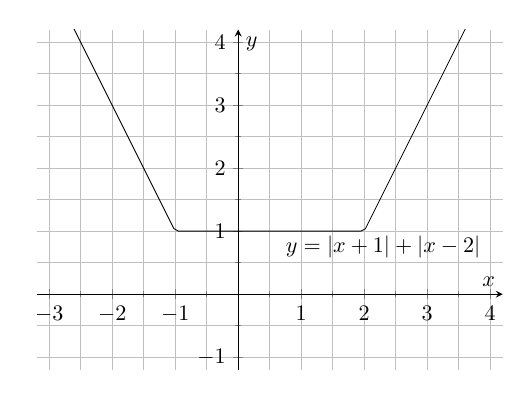
\begin{tikzpicture}[scale = 0.8]
                    \begin{axis}[
                        x=1.0cm,y=1.0cm,
                        axis lines=middle,
                        ymajorgrids=true,
                        xmajorgrids=true,
                        xminorgrids=true,
                        yminorgrids=true,
                        minor tick num=1,
                        xlabel = $x$,
                        ylabel =$y$,
                        xmin=-3.2,
                        xmax=4.2,
                        ymin=-1.2,
                        ymax=4.2,
                        xtick={-3.0,-2.0,...,4.0},
                        ytick={-1.0,0.0,...,4.0},]
                        \draw [samples=100, domain=-3:4] plot(\x,{abs((\x)+1)+abs((\x)-2)-2});
                        \node at (2.3,0.75) {$y=|x+1|+|x-2|$};
                    \end{axis}
                \end{tikzpicture}
            \end{center}
        \end{wrapfigure}

        Nella funzione in figura sono chiaramente visibili tre intervalli: 
        \begin{itemize}
            \item nell'intervallo $]-\infty;-1[$ la funzione è decrescente in senso stretto;
            \item nell'intervallo $]-1;2[$ la funzione è costante, è quindi sia crescente che decrescente in senso lato;
            \item nell'intervallo $]2;+\infty[$ la funzione è crescente in senso stretto.
        \end{itemize}
        Inoltre:
        \begin{itemize}
            \item nell'intervallo $]-\infty;2[$ la funzione è decrescente in senso stretto;
            \item nell'intervallo $]-1;+\infty[$ la funzione è crescente in senso stretto.
        \end{itemize}

        Una funzione è crescente in un intervallo $I$ se e solo se la sua derivata è positiva, decrescente se la derivata è negativa, costante se la derivata è nulla. 
        \begin{definition}[Funzione monotòna]
            Una funzione $f:D\rightarrow C$, con $D\subseteq\R$, si dice \textbf{monotona in senso stretto} in un intervallo $I\subseteq D$ se in quel'intervallo è sempre crescente o sempre decrescente in senso stretto. Analoga definizione può essere data per una funzione monotona in senso lato. 
        \end{definition}
        Nell'esempio precedente la funzione è monotona in senso stretto negli intervalli $]-\infty;-1[$ e $]2;+\infty[$
    \subsection{Funzioni periodiche}
        \begin{definition}
            Una funzione $y=f(x)$ si dice \textbf{periodica} di periodo $T$ (con $T>0$) se, per qualsiasi numero $k\in\Z$, \[f(x)=f(x+kt)\]
        \end{definition}
        Se una funzione è periodica, allora non è iniettiva. 
        \begin{ex}
            La funzione $y=\sin x$ è una funzione periodica di periodo $T=2\pi$
        \end{ex}
        \begin{figure}[h]
            \centering
            \begin{center}
                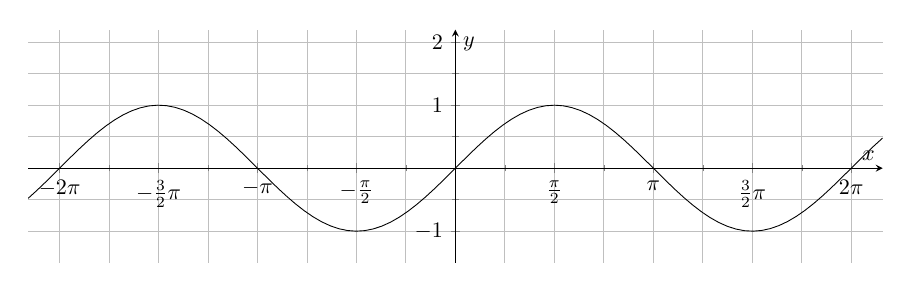
\begin{tikzpicture}[scale = 0.8]
                    \begin{axis}[
                        x=1.0cm,y=1.0cm,
                        axis lines=middle,
                        ymajorgrids=true,
                        xmajorgrids=true,
                        xminorgrids=true,
                        yminorgrids=true,
                        minor tick num=1,
                        xlabel = $x$,
                        ylabel =$y$,
                        xmin=-2*pi-0.5,
                        xmax=2*pi+0.5,
                        ymin=-1.5,
                        ymax=2.2,
                        xtick={-2*pi,-3*pi/2,...,2*pi},
                        xticklabels={$-2\pi$, $-\frac{3}{2}\pi$, $-\pi$,$-\frac{\pi}{2}$,$0$,$\frac{\pi}{2}$,$\pi$, $\frac{3}{2}\pi$, $2\pi$},
                        ytick={-1.0,0.0,...,2.0},]
                        \draw [samples=100, domain=-2*pi-0.5:2*pi+0.5] plot(\x,{sin(((\x))*180/pi)});
                    \end{axis}
                \end{tikzpicture}
            \end{center}
        \end{figure}
    \subsection{Funzioni pari e dispari}
        Si indica con $D$ un sottoinsieme dell'insieme dei numeri reali $\R$ tale che se $x\in D$, allora $-x \in D$.
        \begin{definition}[Funzione pari]
            Data una funzione $y=f(x)$, essa si dice \textit{pari} in $D$ se $\forall x \in D, f(-x)=f(x)$, ovvero la funzione è simmetrica rispetto all'asse delle ordinate.
        \end{definition}
        \begin{definition}[Funzione dispari]
            Data una funzione $y=f(x)$, essa si dice \textit{dispari} in $D$ se $\forall x \in D, f(-x)=-f(x)$, ovvero la funzione è simmetrica rispetto all'origine degli assi.
        \end{definition}
        \textbf{NB.:} Perché una funzione presenti simmetrie deve essere rispettata la condizione necessaria per cui il dominio deve essere simmetrico rispetto a $0$: \[\forall x \in D, -x\in D\]
        \begin{ex}
            La funzione $f(x)=x^2$ è pari, mentre la funzione $g(x)=x^3$ è dispari. Infatti \[f(-x)=(-x)^2=x^2=f(x)\] \[g(-x)=(-x)^3=-x^3=-g(x)\]
        \end{ex}
        \begin{figure}[h]
            \centering
            \begin{subfigure}{0.49\textwidth}
                \begin{center}
                    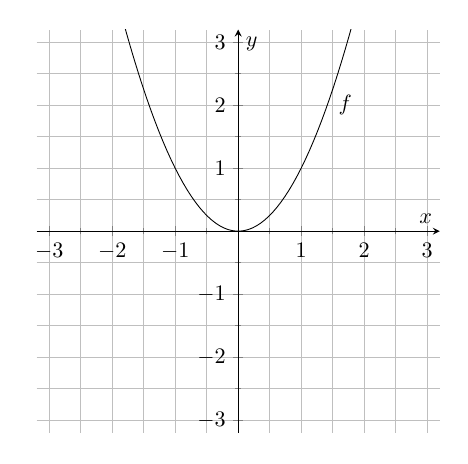
\begin{tikzpicture}[scale = 0.8]
                        \begin{axis}[
                            x=1.0cm,y=1.0cm,
                            axis lines=middle,
                            ymajorgrids=true,
                            xmajorgrids=true,
                            xminorgrids=true,
                            yminorgrids=true,
                            minor tick num=1,
                            xlabel = $x$,
                            ylabel =$y$,
                            xmin=-3.2,
                            xmax=3.2,
                            ymin=-3.2,
                            ymax=3.2,
                            xtick={-3.0,-2.0,...,3.0},
                            ytick={-3.0,-2.0,...,3.0},]
                            \draw [samples=100, domain=-3.2:3.2] plot(\x,{(\x)^2});
                            \node at (1.7,2) {$f$};
                        \end{axis}
                    \end{tikzpicture}
                \end{center}
            \end{subfigure}
            \begin{subfigure}{0.49\textwidth}
                \begin{center}
                    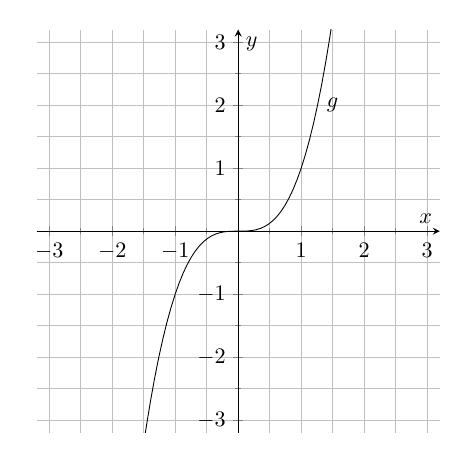
\begin{tikzpicture}[scale = 0.8]
                        \begin{axis}[
                            x=1.0cm,y=1.0cm,
                            axis lines=middle,
                            ymajorgrids=true,
                            xmajorgrids=true,
                            xminorgrids=true,
                            yminorgrids=true,
                            minor tick num=1,
                            xlabel = $x$,
                            ylabel =$y$,
                            xmin=-3.2,
                            xmax=3.2,
                            ymin=-3.2,
                            ymax=3.2,
                            xtick={-3.0,-2.0,...,3.0},
                            ytick={-3.0,-2.0,...,3.0},]
                            \draw [samples=100, domain=-3.2:3.2] plot(\x,{(\x)^3});
                            \node at (1.5,2) {$g$};
                        \end{axis}
                    \end{tikzpicture}
                \end{center}
            \end{subfigure}
        \end{figure}
    \section{Funzioni elementari}
    \subsection{La funzione lineare $y=x$}
        \begin{wrapfigure}[8]{r}{0.20\textwidth}
            \begin{center}
                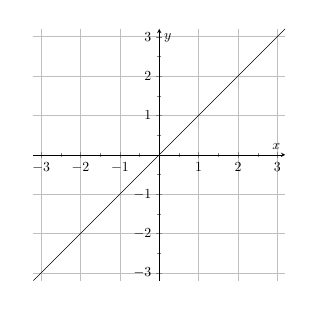
\begin{tikzpicture}[scale = 0.5]
                    \begin{axis}[
                        x=1.0cm,y=1.0cm,
                        axis lines=middle,
                        ymajorgrids=true,
                        xmajorgrids=true,
                        %xminorgrids=true,
                        %yminorgrids=true,
                        minor tick num=1,
                        xlabel = $x$,
                        ylabel =$y$,
                        xmin=-3.2,
                        xmax=3.2,
                        ymin=-3.2,
                        ymax=3.2,
                        xtick={-3.0,-2.0,...,3.0},
                        ytick={-3.0,-2.0,...,3.0},]
                        \draw [samples=100, domain=-3.2:3.2] plot(\x,{(\x)});
                    \end{axis}
                \end{tikzpicture}
            \end{center}
        \end{wrapfigure}
        La funzione lineare è un'equazione polinomiale di primo grado. Il grafico ad essa associato corrisponde ad una retta. Nel caso dela funzione $y=x$ si tratta della bisettrice I-III quadrante. Nell'equaione generica \[y=mx+q\] il parametro $m$, detto coefficiente angolare, identifica la pendenza della retta, mentre il parametro $q$, detto ordinata d'origine, rappresenta il punto di intersezione con l'asse $y$, di coordinate $(0,q)$.
    \subsection{La parabola $y=x^2$}
        \begin{wrapfigure}[8]{r}{0.20\textwidth}
            \begin{center}
                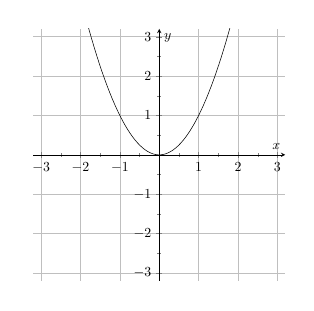
\begin{tikzpicture}[scale = 0.5]
                    \begin{axis}[
                        x=1.0cm,y=1.0cm,
                        axis lines=middle,
                        ymajorgrids=true,
                        xmajorgrids=true,
                        %xminorgrids=true,
                        %yminorgrids=true,
                        minor tick num=1,
                        xlabel = $x$,
                        ylabel =$y$,
                        xmin=-3.2,
                        xmax=3.2,
                        ymin=-3.2,
                        ymax=3.2,
                        xtick={-3.0,-2.0,...,3.0},
                        ytick={-3.0,-2.0,...,3.0},]
                        \draw [samples=100, domain=-3.2:3.2] plot(\x,{(\x)^2});
                    \end{axis}
                \end{tikzpicture}
            \end{center}
        \end{wrapfigure}
        La funzione quadratica è un'equazione polinomiale di secondo grado. Il grafico ad essa associato corrisponde ad una parabola. Nel caso della funzione elementare $y=x^2$ si tratta di una parabola con il vertice nell'origine degli assi e concavità verso l'alto. Nel caso du una parabola generica \[y=ax^2+bx+c\]
        \begin{itemize}
            \item l'asse di simmetria ha equazione $x=-\dfrac{b}{2a}$
            \item il vertice ha coordinate $V\left(-\dfrac{b}{2a};-\dfrac{\Delta}{4a}\right)$
            \item il fuoco ha coordinate $F\left(-\dfrac{b}{2a};\dfrac{1-\Delta}{4a}\right)$
            \item la direttrice ha equazione $y=-\dfrac{1+\Delta}{4a}$
            \item la parabola ha concavità verso l'alto se $a>0$ o verso il basso se $a<0$
        \end{itemize}
    \subsection{L'iperbole equilatera $y=\dfrac{1}{x}$ e la funzione omografica}
        \begin{wrapfigure}[10]{r}{0.2\textwidth}
            \begin{center}
                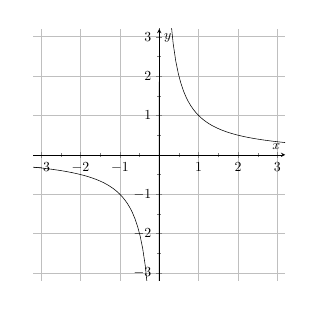
\begin{tikzpicture}[scale = 0.5]
                    \begin{axis}[
                        x=1.0cm,y=1.0cm,
                        axis lines=middle,
                        ymajorgrids=true,
                        xmajorgrids=true,
                        %xminorgrids=true,
                        %yminorgrids=true,
                        minor tick num=1,
                        xlabel = $x$,
                        ylabel =$y$,
                        xmin=-3.2,
                        xmax=3.2,
                        ymin=-3.2,
                        ymax=3.2,
                        xtick={-3.0,-2.0,...,3.0},
                        ytick={-3.0,-2.0,...,3.0},]
                        \draw [samples=100, domain=-3.2:3.2] plot(\x,{1/(\x)});
                    \end{axis}
                \end{tikzpicture}
            \end{center}
        \end{wrapfigure}
        La funzione omografica è caratterizzata dalla relazione di proprzionalità inversa tra le due variabili. L'equazione $y=\frac{k}{x}$ rappresenta un'iperbole equilatera riferita ai propri asintoti con semiasse trasverso $a=\sqrt{2|k|}$, semidistanza focale $c=2\sqrt{|k|}$ e fuochi in $F(\pm\sqrt{2k};\pm\sqrt{2-k})$. Applicando una traslazione di vettore $\vec{v}(-\frac{d}{c},\frac{a}{c})$, si ottiene una funzione omografica generica di equazione \[y=\frac{ax+b}{cx+d}~~~~~~\text{se }c\neq0 \text{ e }ad\neq bc\]\\

        \begin{wrapfigure}[10]{r}{0.2\textwidth}
            \begin{center}
                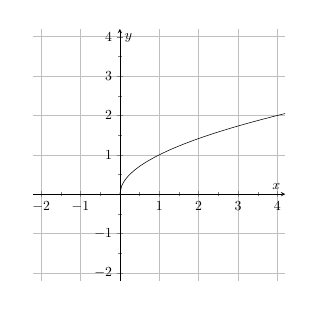
\begin{tikzpicture}[scale = 0.5]
                    \begin{axis}[
                        x=1.0cm,y=1.0cm,
                        axis lines=middle,
                        ymajorgrids=true,
                        xmajorgrids=true,
                        %xminorgrids=true,
                        %yminorgrids=true,
                        minor tick num=1,
                        xlabel = $x$,
                        ylabel =$y$,
                        xmin=-2.2,
                        xmax=4.2,
                        ymin=-2.2,
                        ymax=4.2,
                        xtick={-2.0,-1.0,...,4.0},
                        ytick={-2.0,-1.0,...,4.0},]
                        \draw [samples=100, domain=0:4.2] plot(\x,{sqrt(\x)});
                    \end{axis}
                \end{tikzpicture}
            \end{center}
        \end{wrapfigure}
        Essa a un asintoto verticale di equazione $x=-\dfrac{d}{c}$, un asintoto  orizzontale di equazione $y=\frac{a}{c}$ e di conseguenza ha centro $C(-\frac{d}{c},\frac{a}{c})$. Per ricavare gli altri elementi caratteristici è sufficiente determinare $k=\frac{bc-ad}{c^2}$ e poi applicare un'eventuale traslazione di vettore $\vec{v}$
        \subsection{La funzione irrazionale $y=\sqrt{x}$}
        La funzione irrazionale è l'inversa della funzione quadratica e si ottiene restringendone il dominio e applicando una simmetria rispetto alla biseetrice I-III quadrante. La funzione che si ricava ha dominio $D:[0;+\infty[$ e codominio $C:[0;+\infty[$.
    \subsection{Le funzioni goniometriche}
    \subsubsection{La funzione seno}
        \begin{wrapfigure}{r}{0.5\textwidth}
            \centering
            \begin{center}
                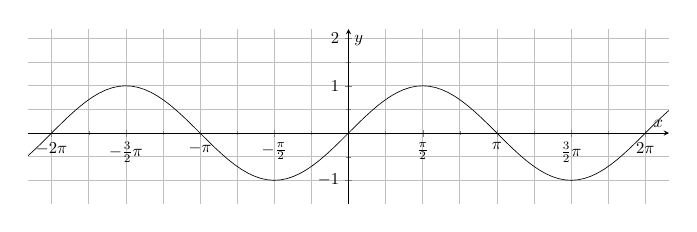
\begin{tikzpicture}[scale = 0.6]
                    \begin{axis}[
                        x=1.0cm,y=1.0cm,
                        axis lines=middle,
                        ymajorgrids=true,
                        xmajorgrids=true,
                        xminorgrids=true,
                        yminorgrids=true,
                        minor tick num=1,
                        xlabel = $x$,
                        ylabel =$y$,
                        xmin=-2*pi-0.5,
                        xmax=2*pi+0.5,
                        ymin=-1.5,
                        ymax=2.2,
                        xtick={-2*pi,-3*pi/2,...,2*pi},
                        xticklabels={$-2\pi$, $-\frac{3}{2}\pi$, $-\pi$,$-\frac{\pi}{2}$,$0$,$\frac{\pi}{2}$,$\pi$, $\frac{3}{2}\pi$, $2\pi$},
                        ytick={-1.0,0.0,...,2.0},]
                        \draw [samples=100, domain=-2*pi-0.5:2*pi+0.5] plot(\x,{sin(((\x))*180/pi)});
                    \end{axis}
                \end{tikzpicture}
            \end{center}
        \end{wrapfigure}
        La funzione seno è una funzione goniometrica trascendente, periodica in $T=2\pi$. Essa ha dominio $D:\R$ e codominio $C:[-1;1]$. Presenta zeri di funzione per $x=k\pi~~(k\in\Z)$, assume valori positivi in $]2k\pi;\pi+2k\pi[$ e negativi altrove. Essa può essere scritta nella forma generica \[y=A\sin(\omega x +\varphi)+B\] dove i parametri rappresentano:
        \begin{itemize}
            \item $A$: ampiezza, rappresenta la dilatazione verticale della funzione, la semidifferenza tra i valori $y$ dei massimi e dei minimi.
            \item $\omega$: pulsazione, è collegata al periodo dalla relazione $\omega =\frac{2\pi}{T}$
            \item $\varphi$: fase, legato alla traslazione orizzontale
            \item $B$: la traslazione verticale
        \end{itemize}
    \subsubsection{La funzione coseno}
        \begin{wrapfigure}[4]{r}{0.5\textwidth}
            \centering
                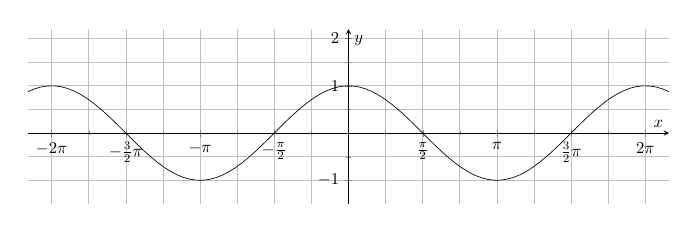
\begin{tikzpicture}[scale = 0.6]
                    \begin{axis}[
                        x=1.0cm,y=1.0cm,
                        axis lines=middle,
                        ymajorgrids=true,
                        xmajorgrids=true,
                        xminorgrids=true,
                        yminorgrids=true,
                        minor tick num=1,
                        xlabel = $x$,
                        ylabel =$y$,
                        xmin=-2*pi-0.5,
                        xmax=2*pi+0.5,
                        ymin=-1.5,
                        ymax=2.2,
                        xtick={-2*pi,-3*pi/2,...,2*pi},
                        xticklabels={$-2\pi$, $-\frac{3}{2}\pi$, $-\pi$,$-\frac{\pi}{2}$,$0$,$\frac{\pi}{2}$,$\pi$, $\frac{3}{2}\pi$, $2\pi$},
                        ytick={-1.0,0.0,...,2.0},]
                        \draw [samples=100, domain=-2*pi-0.5:2*pi+0.5] plot(\x,{cos(((\x))*180/pi)});
                    \end{axis}
                \end{tikzpicture}
        \end{wrapfigure}
        La funzione coseno è una funzione goniometrica trascendente, periodica in $T=2\pi$. Essa ha dominio $D:\R$ e codominio $C:[-1;1]$. Presenta zeri di funzione per $x=\frac{\pi}{2}+k\pi~~(k\in\Z)$, assume valori positivi in $]-\frac{\pi}{2}+k\pi;\frac{\pi}{2}+k\pi[$ e negativi altrove.
    \subsubsection{La funzione tangente}
        \begin{wrapfigure}[4]{r}{0.5\textwidth}
            \centering
                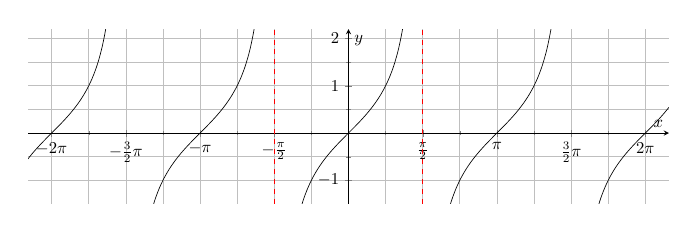
\begin{tikzpicture}[scale = 0.6]
                    \begin{axis}[
                        x=1.0cm,y=1.0cm,
                        axis lines=middle,
                        ymajorgrids=true,
                        xmajorgrids=true,
                        xminorgrids=true,
                        yminorgrids=true,
                        minor tick num=1,
                        xlabel = $x$,
                        ylabel =$y$,
                        xmin=-2*pi-0.5,
                        xmax=2*pi+0.5,
                        ymin=-1.5,
                        ymax=2.2,
                        xtick={-2*pi,-3*pi/2,...,2*pi},
                        xticklabels={$-2\pi$, $-\frac{3}{2}\pi$, $-\pi$,$-\frac{\pi}{2}$,$0$,$\frac{\pi}{2}$,$\pi$, $\frac{3}{2}\pi$, $2\pi$},
                        ytick={-1.0,0.0,...,2.0},]
                        \draw[smooth,samples=30,domain=-0.5*pi+0.1:+0.5*pi-0.1] plot(\x,{tan(((\x))*180/pi)});
                        \draw[smooth,samples=30,domain=-1.5*pi+0.1:-0.5*pi-0.1] plot(\x,{tan(((\x))*180/pi)});
                        \draw[smooth,samples=30,domain=-2.0*pi-0.5:-1.5*pi-0.1] plot(\x,{tan(((\x))*180/pi)});
                        \draw[smooth,samples=30,domain=0.5*pi+0.1:1.5*pi-0.1] plot(\x,{tan(((\x))*180/pi)});
                        \draw[smooth,samples=30,domain=1.5*pi+0.1:2.0*pi+0.5] plot(\x,{tan(((\x))*180/pi)});

                        \draw[dashed, color=red] (0.5*pi,-1.5)--(0.5*pi,2.5);
                        \draw[dashed, color=red] (-0.5*pi,-1.5)--(-0.5*pi,2.5);
                    \end{axis}
                \end{tikzpicture}
        \end{wrapfigure}
        La funzione tangente è una funzione goniometrica trascendente, periodica in $T=\pi$. Essa ha dominio $D:x\neq \frac{\pi}{2}+k\pi~~~(k\in\Z)$ e codominio $C:\R$. Presenta zeri di funzione per $x=k\pi$, assume valori positivi in $]k\pi;\frac{\pi}{2}+2k\pi[$ e negativi altrove. %\newpage
    \subsubsection{La funzione cotangtente}
        \begin{wrapfigure}[4]{r}{0.5\textwidth}
            \centering
                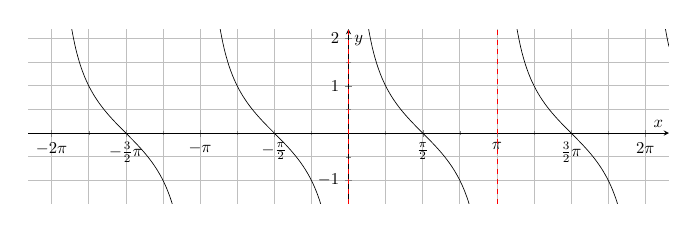
\begin{tikzpicture}[scale = 0.6]
                    \begin{axis}[
                        x=1.0cm,y=1.0cm,
                        axis lines=middle,
                        ymajorgrids=true,
                        xmajorgrids=true,
                        xminorgrids=true,
                        yminorgrids=true,
                        minor tick num=1,
                        xlabel = $x$,
                        ylabel =$y$,
                        xmin=-2*pi-0.5,
                        xmax=2*pi+0.5,
                        ymin=-1.5,
                        ymax=2.2,
                        xtick={-2*pi,-3*pi/2,...,2*pi},
                        xticklabels={$-2\pi$, $-\frac{3}{2}\pi$, $-\pi$,$-\frac{\pi}{2}$,$0$,$\frac{\pi}{2}$,$\pi$, $\frac{3}{2}\pi$, $2\pi$},
                        ytick={-1.0,0.0,...,2.0},]
                        \draw[smooth,samples=30,domain=-1.0*pi+0.1:-0.1] plot(\x,{cot(((\x))*180/pi)});
                        \draw[smooth,samples=30,domain=-2.0*pi+0.1:-1.0*pi-0.1] plot(\x,{cot(((\x))*180/pi)});
                        \draw[smooth,samples=30,domain=-2.0*pi-0.5:-2.0*pi-0.1] plot(\x,{cot(((\x))*180/pi)});
                        \draw[smooth,samples=30,domain=0.1:pi-0.1] plot(\x,{cot(((\x))*180/pi)});
                        \draw[smooth,samples=30,domain=pi+0.1:2.0*pi-0.1] plot(\x,{cot(((\x))*180/pi)});
                        \draw[smooth,samples=30,domain=2.0*pi+0.1:2.0*pi+0.5] plot(\x,{cot(((\x))*180/pi)});

                        \draw[dashed,  color=red] (pi,-1.5)--(pi,2.5);
                        \draw[dashed, thick, color=red] (0,-1.5)--(0,2.5);
                    \end{axis}
                \end{tikzpicture}
        \end{wrapfigure}
        La funzione cotangente è una funzione goniometrica trascendente, periodica in $T=\pi$. Essa ha dominio $D:x\neq k\pi~~~(k\in\Z)$ e codominio $C:\R$. Presenta zeri di funzione per $x= \frac{\pi}{2}+k\pi$, assume valori positivi in $]k\pi;\frac{\pi}{2}+2k\pi[$ e negativi altrove.
    \subsubsection{La funzione arcoseno}
        \begin{wrapfigure}[10]{r}{0.2\textwidth}
                \begin{tikzpicture}[line cap=round,line join=round,>=triangle 45,x=1.0cm,y=1.0cm, scale = 0.6]
                    \begin{axis}[
                    x=1.0cm,y=1.0cm,
                    axis lines=middle,
                    ymajorgrids=true,
                    xmajorgrids=true,
                    xlabel = $x$,
                    ylabel =$y$,
                    xmin=-2.25,
                    xmax=2.25,
                    ymin=-2.5,
                    ymax=2.5,
                    xtick={-2.0,-1.0,...,2.0},
                    ytick={-0.75*pi,-0.5*pi,...,0.75*pi},
                    yticklabels={$-\frac{3}{4}\pi$,$-\frac{\pi}{2}$,$-\frac{\pi}{4}$,$0$,$-\frac{\pi}{4}$,$\frac{\pi}{2}$, $\frac{3}{4}\pi$},
                    ]
                    \clip(-2.,-2.5) rectangle (2.,2.5);
                    \draw (-0.9999999999999991,-1.570796284648048) -- (-0.9999999999999991,-1.570796284648048);
                    \draw (-0.9999999999999991,-1.570796284648048) -- (-0.9950000049999991,-1.4707546632459771);
                    \draw (-0.9950000049999991,-1.4707546632459771) -- (-0.990000009999999,-1.4292569243586009);
                    \draw (-0.990000009999999,-1.4292569243586009) -- (-0.985000014999999,-1.3973740926284461);
                    \draw (-0.985000014999999,-1.3973740926284461) -- (-0.980000019999999,-1.3704615849755784);
                    \draw (-0.980000019999999,-1.3704615849755784) -- (-0.9750000249999989,-1.3467211540018904);
                    \draw (-0.9750000249999989,-1.3467211540018904) -- (-0.9700000299999989,-1.3252309326831408);
                    \draw (-0.9700000299999989,-1.3252309326831408) -- (-0.9650000349999989,-1.3054435106577742);
                    \draw (-0.9650000349999989,-1.3054435106577742) -- (-0.9600000399999988,-1.2870023604437426);
                    \draw (-0.9600000399999988,-1.2870023604437426) -- (-0.9550000449999988,-1.2696599329580787);
                    \draw (-0.9550000449999988,-1.2696599329580787) -- (-0.9500000499999988,-1.2532360576315642);
                    \draw (-0.9500000499999988,-1.2532360576315642) -- (-0.9450000549999987,-1.2375947709339352);
                    \draw (-0.9450000549999987,-1.2375947709339352) -- (-0.9400000599999987,-1.222630481385089);
                    \draw (-0.9400000599999987,-1.222630481385089) -- (-0.9350000649999987,-1.2082592477874345);
                    \draw (-0.9350000649999987,-1.2082592477874345) -- (-0.9300000699999986,-1.1944130349225572);
                    \draw (-0.9300000699999986,-1.1944130349225572) -- (-0.9250000749999986,-1.1810357913829739);
                    \draw (-0.9250000749999986,-1.1810357913829739) -- (-0.9200000799999986,-1.1680806893384255);
                    \draw (-0.9200000799999986,-1.1680806893384255) -- (-0.9150000849999985,-1.1555081313707087);
                    \draw (-0.9150000849999985,-1.1555081313707087) -- (-0.9100000899999985,-1.1432842789224567);
                    \draw (-0.9100000899999985,-1.1432842789224567) -- (-0.9050000949999985,-1.1313799446518304);
                    \draw (-0.9050000949999985,-1.1313799446518304) -- (-0.9000000999999984,-1.1197697444144188);
                    \draw (-0.9000000999999984,-1.1197697444144188) -- (-0.8950001049999984,-1.1084314381666234);
                    \draw (-0.8950001049999984,-1.1084314381666234) -- (-0.8900001099999983,-1.0973454107718383);
                    \draw (-0.8900001099999983,-1.0973454107718383) -- (-0.8850001149999983,-1.0864942580469208);
                    \draw (-0.8850001149999983,-1.0864942580469208) -- (-0.8800001199999983,-1.0758624530996328);
                    \draw (-0.8800001199999983,-1.0758624530996328) -- (-0.8750001249999982,-1.0654360747096856);
                    \draw (-0.8750001249999982,-1.0654360747096856) -- (-0.8700001299999982,-1.055202584212886);
                    \draw (-0.8700001299999982,-1.055202584212886) -- (-0.8650001349999982,-1.0451506407071658);
                    \draw (-0.8650001349999982,-1.0451506407071658) -- (-0.8600001399999981,-1.035269946832199);
                    \draw (-0.8600001399999981,-1.035269946832199) -- (-0.8550001449999981,-1.0255511191601554);
                    \draw (-0.8550001449999981,-1.0255511191601554) -- (-0.8500001499999981,-1.0159855785622856);
                    \draw (-0.8500001499999981,-1.0159855785622856) -- (-0.845000154999998,-1.0065654569136127);
                    \draw (-0.845000154999998,-1.0065654569136127) -- (-0.840000159999998,-0.9972835172557758);
                    \draw (-0.840000159999998,-0.9972835172557758) -- (-0.835000164999998,-0.9881330851193754);
                    \draw (-0.835000164999998,-0.9881330851193754) -- (-0.8300001699999979,-0.9791079891571561);
                    \draw (-0.8300001699999979,-0.9791079891571561) -- (-0.8250001749999979,-0.9702025095906806);
                    \draw (-0.8250001749999979,-0.9702025095906806) -- (-0.8200001799999979,-0.9614113332496197);
                    \draw (-0.8200001799999979,-0.9614113332496197) -- (-0.8150001849999978,-0.9527295142019846);
                    \draw (-0.8150001849999978,-0.9527295142019846) -- (-0.8100001899999978,-0.9441524391486316);
                    \draw (-0.8100001899999978,-0.9441524391486316) -- (-0.8050001949999978,-0.9356757968960285);
                    \draw (-0.8050001949999978,-0.9356757968960285) -- (-0.8000001999999977,-0.9272955513350158);
                    \draw (-0.8000001999999977,-0.9272955513350158) -- (-0.7950002049999977,-0.9190079174458188);
                    \draw (-0.7950002049999977,-0.9190079174458188) -- (-0.7900002099999976,-0.9108093399252589);
                    \draw (-0.7900002099999976,-0.9108093399252589) -- (-0.7850002149999976,-0.9026964740943417);
                    \draw (-0.7850002149999976,-0.9026964740943417) -- (-0.7800002199999976,-0.894666168795833);
                    \draw (-0.7800002199999976,-0.894666168795833) -- (-0.7750002249999975,-0.8867154510341386);
                    \draw (-0.7750002249999975,-0.8867154510341386) -- (-0.7700002299999975,-0.8788415121454257);
                    \draw (-0.7700002299999975,-0.8788415121454257) -- (-0.7650002349999975,-0.8710416953157559);
                    \draw (-0.7650002349999975,-0.8710416953157559) -- (-0.7600002399999974,-0.8633134842901024);
                    \draw (-0.7600002399999974,-0.8633134842901024) -- (-0.7550002449999974,-0.8556544931363114);
                    \draw (-0.7550002449999974,-0.8556544931363114) -- (-0.7500002499999974,-0.848062456946031);
                    \draw (-0.7500002499999974,-0.848062456946031) -- (-0.7450002549999973,-0.8405352233699089);
                    \draw (-0.7450002549999973,-0.8405352233699089) -- (-0.7400002599999973,-0.8330707448973977);
                    \draw (-0.7400002599999973,-0.8330707448973977) -- (-0.7350002649999973,-0.8256670718026775);
                    \draw (-0.7350002649999973,-0.8256670718026775) -- (-0.7300002699999972,-0.8183223456877923);
                    \draw (-0.7300002699999972,-0.8183223456877923) -- (-0.7250002749999972,-0.8110347935623662);
                    \draw (-0.7250002749999972,-0.8110347935623662) -- (-0.7200002799999972,-0.8038027224064028);
                    \draw (-0.7200002799999972,-0.8038027224064028) -- (-0.7150002849999971,-0.7966245141688643);
                    \draw (-0.7150002849999971,-0.7966245141688643) -- (-0.7100002899999971,-0.7894986211600987);
                    \draw (-0.7100002899999971,-0.7894986211600987) -- (-0.7050002949999971,-0.7824235618008739);
                    \draw (-0.7050002949999971,-0.7824235618008739) -- (-0.700000299999997,-0.7753979166948606);
                    \draw (-0.700000299999997,-0.7753979166948606) -- (-0.695000304999997,-0.7684203249949941);
                    \draw (-0.695000304999997,-0.7684203249949941) -- (-0.690000309999997,-0.7614894810372829);
                    \draw (-0.690000309999997,-0.7614894810372829) -- (-0.6850003149999969,-0.7546041312183938);
                    \draw (-0.6850003149999969,-0.7546041312183938) -- (-0.6800003199999969,-0.7477630710957851);
                    \draw (-0.6800003199999969,-0.7477630710957851) -- (-0.6750003249999968,-0.7409651426913004);
                    \draw (-0.6750003249999968,-0.7409651426913004) -- (-0.6700003299999968,-0.7342092319810475);
                    \draw (-0.6700003299999968,-0.7342092319810475) -- (-0.6650003349999968,-0.7274942665560691);
                    \draw (-0.6650003349999968,-0.7274942665560691) -- (-0.6600003399999967,-0.7208192134398131);
                    \draw (-0.6600003399999967,-0.7208192134398131) -- (-0.6550003449999967,-0.7141830770497445);
                    \draw (-0.6550003449999967,-0.7141830770497445) -- (-0.6500003499999967,-0.7075848972916283);
                    \draw (-0.6500003499999967,-0.7075848972916283) -- (-0.6450003549999966,-0.7010237477760809);
                    \draw (-0.6450003549999966,-0.7010237477760809) -- (-0.6400003599999966,-0.6944987341479286);
                    \draw (-0.6400003599999966,-0.6944987341479286) -- (-0.6350003649999966,-0.6880089925197758);
                    \draw (-0.6350003649999966,-0.6880089925197758) -- (-0.6300003699999965,-0.6815536880019362);
                    \draw (-0.6300003699999965,-0.6815536880019362) -- (-0.6250003749999965,-0.675132013321581);
                    \draw (-0.6250003749999965,-0.675132013321581) -- (-0.6200003799999965,-0.6687431875245647);
                    \draw (-0.6200003799999965,-0.6687431875245647) -- (-0.6150003849999964,-0.6623864547539567);
                    \draw (-0.6150003849999964,-0.6623864547539567) -- (-0.6100003899999964,-0.6560610830998023);
                    \draw (-0.6100003899999964,-0.6560610830998023) -- (-0.6050003949999964,-0.6497663635150976);
                    \draw (-0.6050003949999964,-0.6497663635150976) -- (-0.6000003999999963,-0.6435016087933736);
                    \draw (-0.6000003999999963,-0.6435016087933736) -- (-0.5950004049999963,-0.6372661526036532);
                    \draw (-0.5950004049999963,-0.6372661526036532) -- (-0.5900004099999963,-0.631059348578894);
                    \draw (-0.5900004099999963,-0.631059348578894) -- (-0.5850004149999962,-0.6248805694543269);
                    \draw (-0.5850004149999962,-0.6248805694543269) -- (-0.5800004199999962,-0.618729206252388);
                    \draw (-0.5800004199999962,-0.618729206252388) -- (-0.5750004249999962,-0.6126046675111942);
                    \draw (-0.5750004249999962,-0.6126046675111942) -- (-0.5700004299999961,-0.6065063785537455);
                    \draw (-0.5700004299999961,-0.6065063785537455) -- (-0.5650004349999961,-0.600433780795249);
                    \draw (-0.5650004349999961,-0.600433780795249) -- (-0.560000439999996,-0.5943863310861572);
                    \draw (-0.560000439999996,-0.5943863310861572) -- (-0.555000444999996,-0.5883635010886855);
                    \draw (-0.555000444999996,-0.5883635010886855) -- (-0.550000449999996,-0.5823647766847403);
                    \draw (-0.550000449999996,-0.5823647766847403) -- (-0.5450004549999959,-0.5763896574133393);
                    \draw (-0.5450004549999959,-0.5763896574133393) -- (-0.5400004599999959,-0.5704376559357378);
                    \draw (-0.5400004599999959,-0.5704376559357378) -- (-0.5350004649999959,-0.5645082975266067);
                    \draw (-0.5350004649999959,-0.5645082975266067) -- (-0.5300004699999958,-0.5586011195897163);
                    \draw (-0.5300004699999958,-0.5586011195897163) -- (-0.5250004749999958,-0.552715671196695);
                    \draw (-0.5250004749999958,-0.552715671196695) -- (-0.5200004799999958,-0.5468515126475222);
                    \draw (-0.5200004799999958,-0.5468515126475222) -- (-0.5150004849999957,-0.5410082150515105);
                    \draw (-0.5150004849999957,-0.5410082150515105) -- (-0.5100004899999957,-0.5351853599276122);
                    \draw (-0.5100004899999957,-0.5351853599276122) -- (-0.5050004949999957,-0.5293825388229646);
                    \draw (-0.5050004949999957,-0.5293825388229646) -- (-0.5000004999999956,-0.5235993529486592);
                    \draw (-0.5000004999999956,-0.5235993529486592) -- (-0.49500050499999565,-0.517835412831784);
                    \draw (-0.49500050499999565,-0.517835412831784) -- (-0.49000050999999567,-0.5120903379828516);
                    \draw (-0.49000050999999567,-0.5120903379828516) -- (-0.4850005149999957,-0.506363756577782);
                    \draw (-0.4850005149999957,-0.506363756577782) -- (-0.4800005199999957,-0.5006553051536577);
                    \draw (-0.4800005199999957,-0.5006553051536577) -- (-0.47500052499999573,-0.494964628317525);
                    \draw (-0.47500052499999573,-0.494964628317525) -- (-0.47000052999999575,-0.4892913784675504);
                    \draw (-0.47000052999999575,-0.4892913784675504) -- (-0.4650005349999958,-0.4836352155258926);
                    \draw (-0.4650005349999958,-0.4836352155258926) -- (-0.4600005399999958,-0.477995806682684);
                    \draw (-0.4600005399999958,-0.477995806682684) -- (-0.4550005449999958,-0.4723728261505523);
                    \draw (-0.4550005449999958,-0.4723728261505523) -- (-0.45000054999999584,-0.4667659549291493);
                    \draw (-0.45000054999999584,-0.4667659549291493) -- (-0.44500055499999586,-0.4611748805791828);
                    \draw (-0.44500055499999586,-0.4611748805791828) -- (-0.4400005599999959,-0.4555992970054785);
                    \draw (-0.4400005599999959,-0.4555992970054785) -- (-0.4350005649999959,-0.4500389042486249);
                    \draw (-0.4350005649999959,-0.4500389042486249) -- (-0.4300005699999959,-0.4444934082847818);
                    \draw (-0.4300005699999959,-0.4444934082847818) -- (-0.42500057499999594,-0.4389625208332541);
                    \draw (-0.42500057499999594,-0.4389625208332541) -- (-0.42000057999999596,-0.433445959171458);
                    \draw (-0.42000057999999596,-0.433445959171458) -- (-0.415000584999996,-0.42794344595692496);
                    \draw (-0.415000584999996,-0.42794344595692496) -- (-0.410000589999996,-0.4224547090560102);
                    \draw (-0.410000589999996,-0.4224547090560102) -- (-0.405000594999996,-0.4169794813789897);
                    \draw (-0.405000594999996,-0.4169794813789897) -- (-0.40000059999999604,-0.41151750072124793);
                    \draw (-0.40000059999999604,-0.41151750072124793) -- (-0.39500060499999606,-0.4060685096102728);
                    \draw (-0.39500060499999606,-0.4060685096102728) -- (-0.3900006099999961,-0.4006322551581919);
                    \draw (-0.3900006099999961,-0.4006322551581919) -- (-0.3850006149999961,-0.3952084889195962);
                    \draw (-0.3850006149999961,-0.3952084889195962) -- (-0.3800006199999961,-0.3897969667544113);
                    \draw (-0.3800006199999961,-0.3897969667544113) -- (-0.37500062499999615,-0.38439744869558934);
                    \draw (-0.37500062499999615,-0.38439744869558934) -- (-0.37000062999999617,-0.37900969882140617);
                    \draw (-0.37000062999999617,-0.37900969882140617) -- (-0.3650006349999962,-0.37363348513215844);
                    \draw (-0.3650006349999962,-0.37363348513215844) -- (-0.3600006399999962,-0.3682685794310673);
                    \draw (-0.3600006399999962,-0.3682685794310673) -- (-0.35500064499999623,-0.3629147572092041);
                    \draw (-0.35500064499999623,-0.3629147572092041) -- (-0.35000064999999625,-0.3575717975342627);
                    \draw (-0.35000064999999625,-0.3575717975342627) -- (-0.34500065499999627,-0.3522394829430126);
                    \draw (-0.34500065499999627,-0.3522394829430126) -- (-0.3400006599999963,-0.3469175993372734);
                    \draw (-0.3400006599999963,-0.3469175993372734) -- (-0.3350006649999963,-0.3416059358832613);
                    \draw (-0.3350006649999963,-0.3416059358832613) -- (-0.33000066999999633,-0.33630428491416375);
                    \draw (-0.33000066999999633,-0.33630428491416375) -- (-0.32500067499999635,-0.33101244183580536);
                    \draw (-0.32500067499999635,-0.33101244183580536) -- (-0.3200006799999964,-0.3257302050352759);
                    \draw (-0.3200006799999964,-0.3257302050352759) -- (-0.3150006849999964,-0.32045737579239614);
                    \draw (-0.3150006849999964,-0.32045737579239614) -- (-0.3100006899999964,-0.31519375819390316);
                    \draw (-0.3100006899999964,-0.31519375819390316) -- (-0.30500069499999644,-0.3099391590502433);
                    \draw (-0.30500069499999644,-0.3099391590502433) -- (-0.30000069999999646,-0.30469338781486416);
                    \draw (-0.30000069999999646,-0.30469338781486416) -- (-0.2950007049999965,-0.2994562565059045);
                    \draw (-0.2950007049999965,-0.2994562565059045) -- (-0.2900007099999965,-0.29422757963018265);
                    \draw (-0.2900007099999965,-0.29422757963018265) -- (-0.2850007149999965,-0.289007174109391);
                    \draw (-0.2850007149999965,-0.289007174109391) -- (-0.28000071999999654,-0.28379485920840625);
                    \draw (-0.28000071999999654,-0.28379485920840625) -- (-0.27500072499999656,-0.2785904564656312);
                    \draw (-0.27500072499999656,-0.2785904564656312) -- (-0.2700007299999966,-0.27339378962528427);
                    \draw (-0.2700007299999966,-0.27339378962528427) -- (-0.2650007349999966,-0.2682046845715607);
                    \draw (-0.2650007349999966,-0.2682046845715607) -- (-0.2600007399999966,-0.2630229692645892);
                    \draw (-0.2600007399999966,-0.2630229692645892) -- (-0.25500074499999664,-0.2578484736781122);
                    \draw (-0.25500074499999664,-0.2578484736781122) -- (-0.25000074999999666,-0.2526810297388219);
                    \draw (-0.25000074999999666,-0.2526810297388219) -- (-0.24500075499999668,-0.2475204712672856);
                    \draw (-0.24500075499999668,-0.2475204712672856) -- (-0.2400007599999967,-0.24236663392039687);
                    \draw (-0.2400007599999967,-0.24236663392039687) -- (-0.23500076499999673,-0.23721935513529255);
                    \draw (-0.23500076499999673,-0.23721935513529255) -- (-0.23000076999999675,-0.23207847407467716);
                    \draw (-0.23000076999999675,-0.23207847407467716) -- (-0.22500077499999677,-0.22694383157349865);
                    \draw (-0.22500077499999677,-0.22694383157349865) -- (-0.2200007799999968,-0.22181527008692212);
                    \draw (-0.2200007799999968,-0.22181527008692212) -- (-0.2150007849999968,-0.2166926336395496);
                    \draw (-0.2150007849999968,-0.2166926336395496) -- (-0.21000078999999683,-0.21157576777583678);
                    \draw (-0.21000078999999683,-0.21157576777583678) -- (-0.20500079499999685,-0.20646451951165837);
                    \draw (-0.20500079499999685,-0.20646451951165837) -- (-0.20000079999999687,-0.20135873728697656);
                    \draw (-0.20000079999999687,-0.20135873728697656) -- (-0.1950008049999969,-0.19625827091956852);
                    \draw (-0.1950008049999969,-0.19625827091956852) -- (-0.1900008099999969,-0.19116297155976963);
                    \draw (-0.1900008099999969,-0.19116297155976963) -- (-0.18500081499999693,-0.18607269164619222);
                    \draw (-0.18500081499999693,-0.18607269164619222) -- (-0.18000081999999695,-0.18098728486237953);
                    \draw (-0.18000081999999695,-0.18098728486237953) -- (-0.17500082499999697,-0.1759066060943572);
                    \draw (-0.17500082499999697,-0.1759066060943572) -- (-0.170000829999997,-0.17083051138904498);
                    \draw (-0.170000829999997,-0.17083051138904498) -- (-0.16500083499999701,-0.1657588579134932);
                    \draw (-0.16500083499999701,-0.1657588579134932) -- (-0.16000083999999704,-0.1606915039149097);
                    \draw (-0.16000083999999704,-0.1606915039149097) -- (-0.15500084499999706,-0.15562830868144334);
                    \draw (-0.15500084499999706,-0.15562830868144334) -- (-0.15000084999999708,-0.15056913250369275);
                    \draw (-0.15000084999999708,-0.15056913250369275) -- (-0.1450008549999971,-0.1455138366369082);
                    \draw (-0.1450008549999971,-0.1455138366369082) -- (-0.14000085999999712,-0.1404622832638567);
                    \draw (-0.14000085999999712,-0.1404622832638567) -- (-0.13500086499999714,-0.1354143354583213);
                    \draw (-0.13500086499999714,-0.1354143354583213) -- (-0.13000086999999716,-0.13036985714920538);
                    \draw (-0.13000086999999716,-0.13036985714920538) -- (-0.12500087499999718,-0.12532871308521523);
                    \draw (-0.12500087499999718,-0.12532871308521523) -- (-0.12000087999999719,-0.12029076880009315);
                    \draw (-0.12000087999999719,-0.12029076880009315) -- (-0.1150008849999972,-0.11525589057837556);
                    \draw (-0.1150008849999972,-0.11525589057837556) -- (-0.1100008899999972,-0.11022394542165051);
                    \draw (-0.1100008899999972,-0.11022394542165051) -- (-0.10500089499999721,-0.10519480101528984);
                    \draw (-0.10500089499999721,-0.10519480101528984) -- (-0.10000089999999721,-0.10016832569563185);
                    \draw (-0.10000089999999721,-0.10016832569563185) -- (-0.09500090499999722,-0.09514438841759103);
                    \draw (-0.09500090499999722,-0.09514438841759103) -- (-0.09000090999999723,-0.09012285872267181);
                    \draw (-0.09000090999999723,-0.09012285872267181) -- (-0.08500091499999723,-0.08510360670736394);
                    \draw (-0.08500091499999723,-0.08510360670736394) -- (-0.08000091999999724,-0.08008650299189742);
                    \draw (-0.08000091999999724,-0.08008650299189742) -- (-0.07500092499999725,-0.07507141868933569);
                    \draw (-0.07500092499999725,-0.07507141868933569) -- (-0.07000092999999726,-0.07005822537498582);
                    \draw (-0.07000092999999726,-0.07005822537498582) -- (-0.06500093499999726,-0.06504679505610525);
                    \draw (-0.06500093499999726,-0.06504679505610525) -- (-0.06000093999999727,-0.06003700014188448);
                    \draw (-0.06000093999999727,-0.06003700014188448) -- (-0.055000944999997275,-0.05502871341368627);
                    \draw (-0.055000944999997275,-0.05502871341368627) -- (-0.05000094999999728,-0.05002180799552115);
                    \draw (-0.05000094999999728,-0.05002180799552115) -- (-0.04500095499999729,-0.04501615732474046);
                    \draw (-0.04500095499999729,-0.04501615732474046) -- (-0.040000959999997296,-0.040011635122927526);
                    \draw (-0.040000959999997296,-0.040011635122927526) -- (-0.0350009649999973,-0.035008115366968365);
                    \draw (-0.0350009649999973,-0.035008115366968365) -- (-0.030000969999997313,-0.03000547226028324);
                    \draw (-0.030000969999997313,-0.03000547226028324) -- (-0.025000974999997323,-0.025003580204200748);
                    \draw (-0.025000974999997323,-0.025003580204200748) -- (-0.020000979999997334,-0.020002313769456253);
                    \draw (-0.020000979999997334,-0.020002313769456253) -- (-0.015000984999997344,-0.015001547667796579);
                    \draw (-0.015000984999997344,-0.015001547667796579) -- (-0.010000989999997354,-0.01000115672367308);
                    \draw (-0.010000989999997354,-0.01000115672367308) -- (-0.0050009949999973635,-0.005001015846005284);
                    \draw (-0.0050009949999973635,-0.005001015846005284) -- (0.0,0.0);
                    \draw (0.0,0.0) -- (0.004998995000002618,0.004999015821010119);
                    \draw (0.004998995000002618,0.004999015821010119) -- (0.009998990000002608,0.009999156623671035);
                    \draw (0.009998990000002608,0.009999156623671035) -- (0.014998985000002598,0.014999547442764308);
                    \draw (0.014998985000002598,0.014999547442764308) -- (0.019998980000002588,0.02000031336934227);
                    \draw (0.019998980000002588,0.02000031336934227) -- (0.024998975000002577,0.025001579578914135);
                    \draw (0.024998975000002577,0.025001579578914135) -- (0.029998970000002567,0.030003471359682343);
                    \draw (0.029998970000002567,0.030003471359682343) -- (0.03499896500000256,0.03500611414084946);
                    \draw (0.03499896500000256,0.03500611414084946) -- (0.039998960000002554,0.04000963352101343);
                    \draw (0.039998960000002554,0.04000963352101343) -- (0.04499895500000255,0.04501415529666911);
                    \draw (0.04499895500000255,0.04501415529666911) -- (0.04999895000000254,0.050019805490834145);
                    \draw (0.04999895000000254,0.050019805490834145) -- (0.05499894500000253,0.0550267103818173);
                    \draw (0.05499894500000253,0.0550267103818173) -- (0.059998940000002526,0.06003499653214774);
                    \draw (0.059998940000002526,0.06003499653214774) -- (0.06499893500000252,0.06504479081768373);
                    \draw (0.06499893500000252,0.06504479081768373) -- (0.06999893000000251,0.07005622045691962);
                    \draw (0.06999893000000251,0.07005622045691962) -- (0.0749989250000025,0.07506941304051004);
                    \draw (0.0749989250000025,0.07506941304051004) -- (0.0799989200000025,0.08008449656103085);
                    \draw (0.0799989200000025,0.08008449656103085) -- (0.08499891500000249,0.08510159944299614);
                    \draw (0.08499891500000249,0.08510159944299614) -- (0.08999891000000249,0.09012085057315147);
                    \draw (0.08999891000000249,0.09012085057315147) -- (0.09499890500000248,0.09514237933106355);
                    \draw (0.09499890500000248,0.09514237933106355) -- (0.09999890000000247,0.10016631562002691);
                    \draw (0.09999890000000247,0.10016631562002691) -- (0.10499889500000247,0.10519278989830885);
                    \draw (0.10499889500000247,0.10519278989830885) -- (0.10999889000000246,0.11022193321075387);
                    \draw (0.10999889000000246,0.11022193321075387) -- (0.11499888500000245,0.11525387722076977);
                    \draw (0.11499888500000245,0.11525387722076977) -- (0.11999888000000244,0.12028875424271782);
                    \draw (0.11999888000000244,0.12028875424271782) -- (0.12499887500000244,0.1253266972747298);
                    \draw (0.12499887500000244,0.1253266972747298) -- (0.12999887000000243,0.13036784003197582);
                    \draw (0.12999887000000243,0.13036784003197582) -- (0.1349988650000024,0.13541231698040637);
                    \draw (0.1349988650000024,0.13541231698040637) -- (0.1399988600000024,0.1404602633709943);
                    \draw (0.1399988600000024,0.1404602633709943) -- (0.14499885500000237,0.14551181527450122);
                    \draw (0.14499885500000237,0.14551181527450122) -- (0.14999885000000235,0.15056710961679495);
                    \draw (0.14999885000000235,0.15056710961679495) -- (0.15499884500000233,0.15562628421474478);
                    \draw (0.15499884500000233,0.15562628421474478) -- (0.1599988400000023,0.16068947781272208);
                    \draw (0.1599988400000023,0.16068947781272208) -- (0.1649988350000023,0.16575683011973485);
                    \draw (0.1649988350000023,0.16575683011973485) -- (0.16999883000000227,0.17082848184722557);
                    \draw (0.16999883000000227,0.17082848184722557) -- (0.17499882500000224,0.17590457474756227);
                    \draw (0.17499882500000224,0.17590457474756227) -- (0.17999882000000222,0.18098525165325458);
                    \draw (0.17999882000000222,0.18098525165325458) -- (0.1849988150000022,0.1860706565169266);
                    \draw (0.1849988150000022,0.1860706565169266) -- (0.18999881000000218,0.19116093445208013);
                    \draw (0.18999881000000218,0.19116093445208013) -- (0.19499880500000216,0.19625623177468246);
                    \draw (0.19499880500000216,0.19625623177468246) -- (0.19999880000000214,0.20135669604561468);
                    \draw (0.19999880000000214,0.20135669604561468) -- (0.20499879500000212,0.2064624761140173);
                    \draw (0.20499879500000212,0.2064624761140173) -- (0.2099987900000021,0.21157372216157122);
                    \draw (0.2099987900000021,0.21157372216157122) -- (0.21499878500000208,0.21669058574775388);
                    \draw (0.21499878500000208,0.21669058574775388) -- (0.21999878000000206,0.22181321985611152);
                    \draw (0.21999878000000206,0.22181321985611152) -- (0.22499877500000204,0.22694177894159034);
                    \draw (0.22499877500000204,0.22694177894159034) -- (0.22999877000000202,0.2320764189789705);
                    \draw (0.22999877000000202,0.2320764189789705) -- (0.234998765000002,0.23721729751244905);
                    \draw (0.234998765000002,0.23721729751244905) -- (0.23999876000000198,0.24236457370641964);
                    \draw (0.23999876000000198,0.24236457370641964) -- (0.24499875500000196,0.2475184083974983);
                    \draw (0.24499875500000196,0.2475184083974983) -- (0.24999875000000193,0.2526789641478471);
                    \draw (0.24999875000000193,0.2526789641478471) -- (0.2549987450000019,0.2578464052998492);
                    \draw (0.2549987450000019,0.2578464052998492) -- (0.2599987400000019,0.2630208980321915);
                    \draw (0.2599987400000019,0.2630208980321915) -- (0.2649987350000019,0.26820261041741245);
                    \draw (0.2649987350000019,0.26820261041741245) -- (0.26999873000000185,0.2733917124809764);
                    \draw (0.26999873000000185,0.2733917124809764) -- (0.27499872500000183,0.2785883762619369);
                    \draw (0.27499872500000183,0.2785883762619369) -- (0.2799987200000018,0.28379277587525564);
                    \draw (0.2799987200000018,0.28379277587525564) -- (0.2849987150000018,0.28900508757584514);
                    \draw (0.2849987150000018,0.28900508757584514) -- (0.28999871000000177,0.29422548982440694);
                    \draw (0.28999871000000177,0.29422548982440694) -- (0.29499870500000175,0.299454163355141);
                    \draw (0.29499870500000175,0.299454163355141) -- (0.29999870000000173,0.3046912912454036);
                    \draw (0.29999870000000173,0.3046912912454036) -- (0.3049986950000017,0.30993705898739576);
                    \draw (0.3049986950000017,0.30993705898739576) -- (0.3099986900000017,0.31519165456196824);
                    \draw (0.3099986900000017,0.31519165456196824) -- (0.31499868500000167,0.320455268514632);
                    \draw (0.31499868500000167,0.320455268514632) -- (0.31999868000000165,0.3257280940338677);
                    \draw (0.31999868000000165,0.3257280940338677) -- (0.3249986750000016,0.3310103270318321);
                    \draw (0.3249986750000016,0.3310103270318321) -- (0.3299986700000016,0.3363021662275648);
                    \draw (0.3299986700000016,0.3363021662275648) -- (0.3349986650000016,0.3416038132328014);
                    \draw (0.3349986650000016,0.3416038132328014) -- (0.33999866000000156,0.3469154726405067);
                    \draw (0.33999866000000156,0.3469154726405067) -- (0.34499865500000154,0.3522373521162455);
                    \draw (0.34499865500000154,0.3522373521162455) -- (0.3499986500000015,0.35756966249251565);
                    \draw (0.3499986500000015,0.35756966249251565) -- (0.3549986450000015,0.36291261786617174);
                    \draw (0.3549986450000015,0.36291261786617174) -- (0.3599986400000015,0.36826643569907785);
                    \draw (0.3599986400000015,0.36826643569907785) -- (0.36499863500000146,0.37363133692213113);
                    \draw (0.36499863500000146,0.37363133692213113) -- (0.36999863000000144,0.37900754604280756);
                    \draw (0.36999863000000144,0.37900754604280756) -- (0.3749986250000014,0.38439529125638816);
                    \draw (0.3749986250000014,0.38439529125638816) -- (0.3799986200000014,0.38979480456103155);
                    \draw (0.3799986200000014,0.38979480456103155) -- (0.3849986150000014,0.39520632187686877);
                    \draw (0.3849986150000014,0.39520632187686877) -- (0.38999861000000136,0.40063008316930426);
                    \draw (0.38999861000000136,0.40063008316930426) -- (0.39499860500000133,0.40606633257671704);
                    \draw (0.39499860500000133,0.40606633257671704) -- (0.3999986000000013,0.41151531854276696);
                    \draw (0.3999986000000013,0.41151531854276696) -- (0.4049985950000013,0.4169772939535214);
                    \draw (0.4049985950000013,0.4169772939535214) -- (0.4099985900000013,0.4224525162796294);
                    \draw (0.4099985900000013,0.4224525162796294) -- (0.41499858500000125,0.42794124772378345);
                    \draw (0.41499858500000125,0.42794124772378345) -- (0.41999858000000123,0.4334437553737222);
                    \draw (0.41999858000000123,0.4334437553737222) -- (0.4249985750000012,0.4389603113610403);
                    \draw (0.4249985750000012,0.4389603113610403) -- (0.4299985700000012,0.44449119302608897);
                    \draw (0.4299985700000012,0.44449119302608897) -- (0.43499856500000117,0.4500366830892648);
                    \draw (0.43499856500000117,0.4500366830892648) -- (0.43999856000000115,0.45559706982900317);
                    \draw (0.43999856000000115,0.45559706982900317) -- (0.44499855500000113,0.461172647266809);
                    \draw (0.44499855500000113,0.461172647266809) -- (0.4499985500000011,0.4667637153596801);
                    \draw (0.4499985500000011,0.4667637153596801) -- (0.4549985450000011,0.4723705802002953);
                    \draw (0.4549985450000011,0.4723705802002953) -- (0.45999854000000107,0.4779935542253665);
                    \draw (0.45999854000000107,0.4779935542253665) -- (0.46499853500000105,0.4836329564325728);
                    \draw (0.46499853500000105,0.4836329564325728) -- (0.469998530000001,0.4892891126065253);
                    \draw (0.469998530000001,0.4892891126065253) -- (0.474998525000001,0.49496235555423435);
                    \draw (0.474998525000001,0.49496235555423435) -- (0.479998520000001,0.5006530253505833);
                    \draw (0.479998520000001,0.5006530253505833) -- (0.48499851500000096,0.5063614695943436);
                    \draw (0.48499851500000096,0.5063614695943436) -- (0.48999851000000094,0.5120880436752976);
                    \draw (0.48999851000000094,0.5120880436752976) -- (0.4949985050000009,0.5178331110530773);
                    \draw (0.4949985050000009,0.5178331110530773) -- (0.4999985000000009,0.5235970435483583);
                    \draw (0.4999985000000009,0.5235970435483583) -- (0.5049984950000009,0.5293802216470994);
                    \draw (0.5049984950000009,0.5293802216470994) -- (0.509998490000001,0.5351830348185534);
                    \draw (0.509998490000001,0.5351830348185534) -- (0.514998485000001,0.5410058818478343);
                    \draw (0.514998485000001,0.5410058818478343) -- (0.519998480000001,0.5468491711838672);
                    \draw (0.519998480000001,0.5468491711838672) -- (0.5249984750000011,0.5527133213036135);
                    \draw (0.5249984750000011,0.5527133213036135) -- (0.5299984700000011,0.5585987610935182);
                    \draw (0.5299984700000011,0.5585987610935182) -- (0.5349984650000011,0.5645059302491957);
                    \draw (0.5349984650000011,0.5645059302491957) -- (0.5399984600000012,0.5704352796944396);
                    \draw (0.5399984600000012,0.5704352796944396) -- (0.5449984550000012,0.5763872720207218);
                    \draw (0.5449984550000012,0.5763872720207218) -- (0.5499984500000012,0.5823623819484248);
                    \draw (0.5499984500000012,0.5823623819484248) -- (0.5549984450000013,0.5883610968111477);
                    \draw (0.5549984450000013,0.5883610968111477) -- (0.5599984400000013,0.5943839170645187);
                    \draw (0.5599984400000013,0.5943839170645187) -- (0.5649984350000014,0.6004313568210577);
                    \draw (0.5649984350000014,0.6004313568210577) -- (0.5699984300000014,0.6065039444127456);
                    \draw (0.5699984300000014,0.6065039444127456) -- (0.5749984250000014,0.6126022229830828);
                    \draw (0.5749984250000014,0.6126022229830828) -- (0.5799984200000015,0.6187267511105583);
                    \draw (0.5799984200000015,0.6187267511105583) -- (0.5849984150000015,0.6248781034655999);
                    \draw (0.5849984150000015,0.6248781034655999) -- (0.5899984100000015,0.631056871503233);
                    \draw (0.5899984100000015,0.631056871503233) -- (0.5949984050000016,0.6372636641938636);
                    \draw (0.5949984050000016,0.6372636641938636) -- (0.5999984000000016,0.6434991087947863);
                    \draw (0.5999984000000016,0.6434991087947863) -- (0.6049983950000016,0.6497638516652336);
                    \draw (0.6049983950000016,0.6497638516652336) -- (0.6099983900000017,0.6560585591280177);
                    \draw (0.6099983900000017,0.6560585591280177) -- (0.6149983850000017,0.6623839183810687);
                    \draw (0.6149983850000017,0.6623839183810687) -- (0.6199983800000017,0.6687406384624535);
                    \draw (0.6199983800000017,0.6687406384624535) -- (0.6249983750000018,0.6751294512727691);
                    \draw (0.6249983750000018,0.6751294512727691) -- (0.6299983700000018,0.6815511126591424);
                    \draw (0.6299983700000018,0.6815511126591424) -- (0.6349983650000018,0.6880064035654401);
                    \draw (0.6349983650000018,0.6880064035654401) -- (0.6399983600000019,0.6944961312537098);
                    \draw (0.6399983600000019,0.6944961312537098) -- (0.6449983550000019,0.7010211306023204);
                    \draw (0.6449983550000019,0.7010211306023204) -- (0.649998350000002,0.7075822654867809);
                    \draw (0.649998350000002,0.7075822654867809) -- (0.654998345000002,0.7141804302497711);
                    \draw (0.654998345000002,0.7141804302497711) -- (0.659998340000002,0.7208165512675344);
                    \draw (0.659998340000002,0.7208165512675344) -- (0.664998335000002,0.727491588620475);
                    \draw (0.664998335000002,0.727491588620475) -- (0.6699983300000021,0.7342065378765602);
                    \draw (0.6699983300000021,0.7342065378765602) -- (0.6749983250000021,0.7409624319969861);
                    \draw (0.6749983250000021,0.7409624319969861) -- (0.6799983200000022,0.7477603433745106);
                    \draw (0.6799983200000022,0.7477603433745106) -- (0.6849983150000022,0.7546013860159231);
                    \draw (0.6849983150000022,0.7546013860159231) -- (0.6899983100000022,0.7614867178813084);
                    \draw (0.6899983100000022,0.7614867178813084) -- (0.6949983050000023,0.7684175433940966);
                    \draw (0.6949983050000023,0.7684175433940966) -- (0.6999983000000023,0.7753951161373906);
                    \draw (0.6999983000000023,0.7753951161373906) -- (0.7049982950000023,0.7824207417537492);
                    \draw (0.7049982950000023,0.7824207417537492) -- (0.7099982900000024,0.7894957810675076);
                    \draw (0.7099982900000024,0.7894957810675076) -- (0.7149982850000024,0.7966216534508678);
                    \draw (0.7149982850000024,0.7966216534508678) -- (0.7199982800000024,0.803799840457424);
                    \draw (0.7199982800000024,0.803799840457424) -- (0.7249982750000025,0.8110318897495568);
                    \draw (0.7249982750000025,0.8110318897495568) -- (0.7299982700000025,0.8183194193492632);
                    \draw (0.7299982700000025,0.8183194193492632) -- (0.7349982650000025,0.8256641222455796);
                    \draw (0.7349982650000025,0.8256641222455796) -- (0.7399982600000026,0.8330677713958375);
                    \draw (0.7399982600000026,0.8330677713958375) -- (0.7449982550000026,0.84053222516268);
                    \draw (0.7449982550000026,0.84053222516268) -- (0.7499982500000026,0.8480594332341426);
                    \draw (0.7499982500000026,0.8480594332341426) -- (0.7549982450000027,0.8556514430802904);
                    \draw (0.7549982450000027,0.8556514430802904) -- (0.7599982400000027,0.863310407007044);
                    \draw (0.7599982400000027,0.863310407007044) -- (0.7649982350000027,0.8710385898760915);
                    \draw (0.7649982350000027,0.8710385898760915) -- (0.7699982300000028,0.8788383775693771);
                    \draw (0.7699982300000028,0.8788383775693771) -- (0.7749982250000028,0.886712286287818);
                    \draw (0.7749982250000028,0.886712286287818) -- (0.7799982200000029,0.8946629727869464);
                    \draw (0.7799982200000029,0.8946629727869464) -- (0.7849982150000029,0.902693245667444);
                    \draw (0.7849982150000029,0.902693245667444) -- (0.7899982100000029,0.9108060778565028);
                    \draw (0.7899982100000029,0.9108060778565028) -- (0.794998205000003,0.9190046204371305);
                    \draw (0.794998205000003,0.9190046204371305) -- (0.799998200000003,0.9272922180076172);
                    \draw (0.799998200000003,0.9272922180076172) -- (0.804998195000003,0.9356724257832165);
                    \draw (0.804998195000003,0.9356724257832165) -- (0.8099981900000031,0.9441490286877062);
                    \draw (0.8099981900000031,0.9441490286877062) -- (0.8149981850000031,0.9527260627252004);
                    \draw (0.8149981850000031,0.9527260627252004) -- (0.8199981800000031,0.9614078389740118);
                    \draw (0.8199981800000031,0.9614078389740118) -- (0.8249981750000032,0.9701989706065902);
                    \draw (0.8249981750000032,0.9701989706065902) -- (0.8299981700000032,0.9791044034152461);
                    \draw (0.8299981700000032,0.9791044034152461) -- (0.8349981650000032,0.988129450415885);
                    \draw (0.8349981650000032,0.988129450415885) -- (0.8399981600000033,0.9972798312157161);
                    \draw (0.8399981600000033,0.9972798312157161) -- (0.8449981550000033,1.0065617169715375);
                    \draw (0.8449981550000033,1.0065617169715375) -- (0.8499981500000033,1.0159817819401975);
                    \draw (0.8499981500000033,1.0159817819401975) -- (0.8549981450000034,1.0255472628420084);
                    \draw (0.8549981450000034,1.0255472628420084) -- (0.8599981400000034,1.0352660275343328);
                    \draw (0.8599981400000034,1.0352660275343328) -- (0.8649981350000034,1.045146654843851);
                    \draw (0.8649981350000034,1.045146654843851) -- (0.8699981300000035,1.0551985278559546);
                    \draw (0.8699981300000035,1.0551985278559546) -- (0.8749981250000035,1.0654319435409558);
                    \draw (0.8749981250000035,1.0654319435409558) -- (0.8799981200000035,1.0758582423544925);
                    \draw (0.8799981200000035,1.0758582423544925) -- (0.8849981150000036,1.086489962446978);
                    \draw (0.8849981150000036,1.086489962446978) -- (0.8899981100000036,1.0973410244439288);
                    \draw (0.8899981100000036,1.0973410244439288) -- (0.8949981050000037,1.108426954544644);
                    \draw (0.8949981050000037,1.108426954544644) -- (0.8999981000000037,1.119765156119314);
                    \draw (0.8999981000000037,1.119765156119314) -- (0.9049980950000037,1.131375243343483);
                    \draw (0.9049980950000037,1.131375243343483) -- (0.9099980900000038,1.1432794551150052);
                    \draw (0.9099980900000038,1.1432794551150052) -- (0.9149980850000038,1.155503174199613);
                    \draw (0.9149980850000038,1.155503174199613) -- (0.9199980800000038,1.168075586262928);
                    \draw (0.9199980800000038,1.168075586262928) -- (0.9249980750000039,1.1810305278006221);
                    \draw (0.9249980750000039,1.1810305278006221) -- (0.9299980700000039,1.1944075936617877);
                    \draw (0.9299980700000039,1.1944075936617877) -- (0.9349980650000039,1.2082536084275208);
                    \draw (0.9349980650000039,1.2082536084275208) -- (0.939998060000004,1.2226246193257857);
                    \draw (0.939998060000004,1.2226246193257857) -- (0.944998055000004,1.237588656092194);
                    \draw (0.944998055000004,1.237588656092194) -- (0.949998050000004,1.2532296525647162);
                    \draw (0.949998050000004,1.2532296525647162) -- (0.9549980450000041,1.2696531900714993);
                    \draw (0.9549980450000041,1.2696531900714993) -- (0.9599980400000041,1.2869952176705812);
                    \draw (0.9599980400000041,1.2869952176705812) -- (0.9649980350000041,1.3054358844468155);
                    \draw (0.9649980350000041,1.3054358844468155) -- (0.9699980300000042,1.3252227059134367);
                    \draw (0.9699980300000042,1.3252227059134367) -- (0.9749980250000042,1.346712153471992);
                    \draw (0.9749980250000042,1.346712153471992) -- (0.9799980200000042,1.370451534841187);
                    \draw (0.9799980200000042,1.370451534841187) -- (0.9849980150000043,1.3973625024543763);
                    \draw (0.9849980150000043,1.3973625024543763) -- (0.9899980100000043,1.429242747432734);
                    \draw (0.9899980100000043,1.429242747432734) -- (0.9949980050000043,1.470734640186159);
                    \end{axis}
                    \end{tikzpicture}
        \end{wrapfigure}
        La funzione arcoseno (in figura) è l'inversa della funzione seno. Per poter invertire questa funzione è necessario restringerne il dominio a $[-\frac{\pi}{2};\frac{\pi}{2}]$ e il codominio a $[-1;1]$. di conseguenza la funzione arcoseno ha dominio $D: [-1;1]$ e codominio $C:[-\frac{\pi}{2};\frac{\pi}{2}]$. Essa presenta inoltre un solo zero di funzione per $x=0$.
    \subsubsection{La funzione arcocoseno}
        Analogamente alla funzione arcoseno, la funzione arcocoseno è l'inversa del coseno. Anche in questo caso il dominio e il codominio devono essere ristretti a $D': [0;\pi]$ e $C': [-1;1]$. di conseguenza la funzione arcoseno ha dominio $D: [-1;1]$ e codominio $C:[0;\pi]$. Essa presenta inoltre un solo zero di funzione per $x=-1$. Il grafico consiste in una traslazione verso l'alto di $\pi$ unità del grafico della funzione arcoseno.
    \subsubsection{La funzione arcotangente}
        \begin{wrapfigure}{r}{0.5\textwidth}
            \centering
                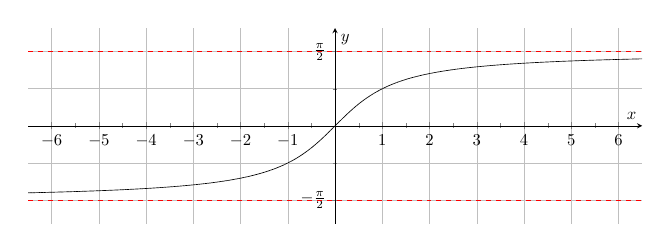
\begin{tikzpicture}[scale = 0.6]
                    \begin{axis}[
                        x=1.0cm,y=1.0cm,
                        axis lines=middle,
                        ymajorgrids=true,
                        xmajorgrids=true,
                        %xminorgrids=true,
                        yminorgrids=true,
                        minor tick num=1,
                        xlabel = $x$,
                        ylabel =$y$,
                        xmin=-6.5,
                        xmax=6.5,
                        ymin=-0.5*pi-0.5,
                        ymax=0.5*pi+0.5,
                        xtick={-6.0,-5.0,...,6.0},
                        ytick={-0.5*pi,0,...,0.5*pi},
                        yticklabels={$-\frac{\pi}{2}$,$0$,$\frac{\pi}{2}$},]

                        \draw[dashed, color=red] (-6.5,0.5*pi)--(6.5,0.5*pi);
                        \draw[dashed, color=red] (-6.5,-0.5*pi)--(6.5,-0.5*pi);

                        \clip(-6.5,-1.6) rectangle (6.5,1.6);
                        \draw (-6.5,-1.4181469983996315) -- (-6.5,-1.4181469983996315);
                        \draw (-6.5,-1.4181469983996315) -- (-6.4675,-1.4173918650878474);
                        \draw (-6.4675,-1.4173918650878474) -- (-6.4350000000000005,-1.4166292831444403);
                        \draw (-6.4350000000000005,-1.4166292831444403) -- (-6.402500000000001,-1.415859142713462);
                        \draw (-6.402500000000001,-1.415859142713462) -- (-6.370000000000001,-1.4150813317862707);
                        \draw (-6.370000000000001,-1.4150813317862707) -- (-6.337500000000001,-1.414295736149008);
                        \draw (-6.337500000000001,-1.414295736149008) -- (-6.3050000000000015,-1.4135022393285461);
                        \draw (-6.3050000000000015,-1.4135022393285461) -- (-6.272500000000002,-1.4127007225368495);
                        \draw (-6.272500000000002,-1.4127007225368495) -- (-6.240000000000002,-1.4118910646137035);
                        \draw (-6.240000000000002,-1.4118910646137035) -- (-6.207500000000002,-1.4110731419677478);
                        \draw (-6.207500000000002,-1.4110731419677478) -- (-6.1750000000000025,-1.4102468285157603);
                        \draw (-6.1750000000000025,-1.4102468285157603) -- (-6.142500000000003,-1.409411995620132);
                        \draw (-6.142500000000003,-1.409411995620132) -- (-6.110000000000003,-1.4085685120244655);
                        \draw (-6.110000000000003,-1.4085685120244655) -- (-6.077500000000003,-1.4077162437872364);
                        \draw (-6.077500000000003,-1.4077162437872364) -- (-6.0450000000000035,-1.4068550542134495);
                        \draw (-6.0450000000000035,-1.4068550542134495) -- (-6.012500000000004,-1.4059848037842175);
                        \draw (-6.012500000000004,-1.4059848037842175) -- (-5.980000000000004,-1.4051053500841904);
                        \draw (-5.980000000000004,-1.4051053500841904) -- (-5.947500000000004,-1.4042165477267579);
                        \draw (-5.947500000000004,-1.4042165477267579) -- (-5.9150000000000045,-1.403318248276949);
                        \draw (-5.9150000000000045,-1.403318248276949) -- (-5.882500000000005,-1.4024103001719435);
                        \draw (-5.882500000000005,-1.4024103001719435) -- (-5.850000000000005,-1.4014925486391092);
                        \draw (-5.850000000000005,-1.4014925486391092) -- (-5.817500000000005,-1.4005648356114806);
                        \draw (-5.817500000000005,-1.4005648356114806) -- (-5.7850000000000055,-1.3996269996405784);
                        \draw (-5.7850000000000055,-1.3996269996405784) -- (-5.752500000000006,-1.3986788758064812);
                        \draw (-5.752500000000006,-1.3986788758064812) -- (-5.720000000000006,-1.3977202956250439);
                        \draw (-5.720000000000006,-1.3977202956250439) -- (-5.687500000000006,-1.396751086952158);
                        \draw (-5.687500000000006,-1.396751086952158) -- (-5.6550000000000065,-1.3957710738849496);
                        \draw (-5.6550000000000065,-1.3957710738849496) -- (-5.622500000000007,-1.394780076659793);
                        \draw (-5.622500000000007,-1.394780076659793) -- (-5.590000000000007,-1.3937779115470315);
                        \draw (-5.590000000000007,-1.3937779115470315) -- (-5.557500000000007,-1.3927643907422729);
                        \draw (-5.557500000000007,-1.3927643907422729) -- (-5.5250000000000075,-1.3917393222541365);
                        \draw (-5.5250000000000075,-1.3917393222541365) -- (-5.492500000000008,-1.390702509788316);
                        \draw (-5.492500000000008,-1.390702509788316) -- (-5.460000000000008,-1.389653752627819);
                        \draw (-5.460000000000008,-1.389653752627819) -- (-5.427500000000008,-1.3885928455092331);
                        \draw (-5.427500000000008,-1.3885928455092331) -- (-5.3950000000000085,-1.3875195784948755);
                        \draw (-5.3950000000000085,-1.3875195784948755) -- (-5.362500000000009,-1.3864337368406556);
                        \draw (-5.362500000000009,-1.3864337368406556) -- (-5.330000000000009,-1.3853351008594963);
                        \draw (-5.330000000000009,-1.3853351008594963) -- (-5.297500000000009,-1.3842234457801315);
                        \draw (-5.297500000000009,-1.3842234457801315) -- (-5.2650000000000095,-1.3830985416011055);
                        \draw (-5.2650000000000095,-1.3830985416011055) -- (-5.23250000000001,-1.3819601529397847);
                        \draw (-5.23250000000001,-1.3819601529397847) -- (-5.20000000000001,-1.3808080388761812);
                        \draw (-5.20000000000001,-1.3808080388761812) -- (-5.16750000000001,-1.379641952791387);
                        \draw (-5.16750000000001,-1.379641952791387) -- (-5.1350000000000104,-1.3784616422004017);
                        \draw (-5.1350000000000104,-1.3784616422004017) -- (-5.102500000000011,-1.3772668485791295);
                        \draw (-5.102500000000011,-1.3772668485791295) -- (-5.070000000000011,-1.3760573071853115);
                        \draw (-5.070000000000011,-1.3760573071853115) -- (-5.037500000000011,-1.3748327468731467);
                        \draw (-5.037500000000011,-1.3748327468731467) -- (-5.005000000000011,-1.373592889901346);
                        \draw (-5.005000000000011,-1.373592889901346) -- (-4.972500000000012,-1.372337451734352);
                        \draw (-4.972500000000012,-1.372337451734352) -- (-4.940000000000012,-1.3710661408364413);
                        \draw (-4.940000000000012,-1.3710661408364413) -- (-4.907500000000012,-1.3697786584584186);
                        \draw (-4.907500000000012,-1.3697786584584186) -- (-4.875000000000012,-1.3684746984165934);
                        \draw (-4.875000000000012,-1.3684746984165934) -- (-4.842500000000013,-1.367153946863719);
                        \draw (-4.842500000000013,-1.367153946863719) -- (-4.810000000000013,-1.3658160820515561);
                        \draw (-4.810000000000013,-1.3658160820515561) -- (-4.777500000000013,-1.3644607740847097);
                        \draw (-4.777500000000013,-1.3644607740847097) -- (-4.745000000000013,-1.3630876846653692);
                        \draw (-4.745000000000013,-1.3630876846653692) -- (-4.712500000000014,-1.3616964668285658);
                        \draw (-4.712500000000014,-1.3616964668285658) -- (-4.680000000000014,-1.3602867646675412);
                        \draw (-4.680000000000014,-1.3602867646675412) -- (-4.647500000000014,-1.3588582130488036);
                        \draw (-4.647500000000014,-1.3588582130488036) -- (-4.615000000000014,-1.3574104373164266);
                        \draw (-4.615000000000014,-1.3574104373164266) -- (-4.582500000000015,-1.3559430529851235);
                        \draw (-4.582500000000015,-1.3559430529851235) -- (-4.550000000000015,-1.3544556654216067);
                        \draw (-4.550000000000015,-1.3544556654216067) -- (-4.517500000000015,-1.352947869513723);
                        \draw (-4.517500000000015,-1.352947869513723) -- (-4.485000000000015,-1.3514192493268211);
                        \draw (-4.485000000000015,-1.3514192493268211) -- (-4.452500000000016,-1.3498693777467925);
                        \draw (-4.452500000000016,-1.3498693777467925) -- (-4.420000000000016,-1.348297816109187);
                        \draw (-4.420000000000016,-1.348297816109187) -- (-4.387500000000016,-1.3467041138137854);
                        \draw (-4.387500000000016,-1.3467041138137854) -- (-4.355000000000016,-1.3450878079239736);
                        \draw (-4.355000000000016,-1.3450878079239736) -- (-4.322500000000017,-1.343448422750233);
                        \draw (-4.322500000000017,-1.343448422750233) -- (-4.290000000000017,-1.341785469417027);
                        \draw (-4.290000000000017,-1.341785469417027) -- (-4.257500000000017,-1.340098445412325);
                        \draw (-4.257500000000017,-1.340098445412325) -- (-4.225000000000017,-1.3383868341189702);
                        \draw (-4.225000000000017,-1.3383868341189702) -- (-4.192500000000018,-1.336650104327055);
                        \draw (-4.192500000000018,-1.336650104327055) -- (-4.160000000000018,-1.334887709726426);
                        \draw (-4.160000000000018,-1.334887709726426) -- (-4.127500000000018,-1.3330990883783898);
                        \draw (-4.127500000000018,-1.3330990883783898) -- (-4.095000000000018,-1.331283662165657);
                        \draw (-4.095000000000018,-1.331283662165657) -- (-4.062500000000019,-1.3294408362194938);
                        \draw (-4.062500000000019,-1.3294408362194938) -- (-4.030000000000019,-1.3275699983230118);
                        \draw (-4.030000000000019,-1.3275699983230118) -- (-3.9975000000000187,-1.3256705182894604);
                        \draw (-3.9975000000000187,-1.3256705182894604) -- (-3.9650000000000185,-1.3237417473143374);
                        \draw (-3.9650000000000185,-1.3237417473143374) -- (-3.9325000000000183,-1.3217830173000569);
                        \draw (-3.9325000000000183,-1.3217830173000569) -- (-3.900000000000018,-1.319793640151863);
                        \draw (-3.900000000000018,-1.319793640151863) -- (-3.867500000000018,-1.3177729070435944);
                        \draw (-3.867500000000018,-1.3177729070435944) -- (-3.8350000000000177,-1.31572008765184);
                        \draw (-3.8350000000000177,-1.31572008765184) -- (-3.8025000000000175,-1.3136344293569449);
                        \draw (-3.8025000000000175,-1.3136344293569449) -- (-3.7700000000000173,-1.3115151564092409);
                        \draw (-3.7700000000000173,-1.3115151564092409) -- (-3.737500000000017,-1.309361469058795);
                        \draw (-3.737500000000017,-1.309361469058795) -- (-3.705000000000017,-1.3071725426468694);
                        \draw (-3.705000000000017,-1.3071725426468694) -- (-3.6725000000000168,-1.3049475266571977);
                        \draw (-3.6725000000000168,-1.3049475266571977) -- (-3.6400000000000166,-1.3026855437250706);
                        \draw (-3.6400000000000166,-1.3026855437250706) -- (-3.6075000000000164,-1.300385688602126);
                        \draw (-3.6075000000000164,-1.300385688602126) -- (-3.575000000000016,-1.2980470270746127);
                        \draw (-3.575000000000016,-1.2980470270746127) -- (-3.542500000000016,-1.2956685948327833);
                        \draw (-3.542500000000016,-1.2956685948327833) -- (-3.5100000000000158,-1.293249396288946);
                        \draw (-3.5100000000000158,-1.293249396288946) -- (-3.4775000000000156,-1.290788403341557);
                        \draw (-3.4775000000000156,-1.290788403341557) -- (-3.4450000000000154,-1.2882845540826133);
                        \draw (-3.4450000000000154,-1.2882845540826133) -- (-3.412500000000015,-1.2857367514454303);
                        \draw (-3.412500000000015,-1.2857367514454303) -- (-3.380000000000015,-1.283143861789756);
                        \draw (-3.380000000000015,-1.283143861789756) -- (-3.347500000000015,-1.2805047134209833);
                        \draw (-3.347500000000015,-1.2805047134209833) -- (-3.3150000000000146,-1.2778180950400593);
                        \draw (-3.3150000000000146,-1.2778180950400593) -- (-3.2825000000000144,-1.2750827541204997);
                        \draw (-3.2825000000000144,-1.2750827541204997) -- (-3.250000000000014,-1.2722973952087187);
                        \draw (-3.250000000000014,-1.2722973952087187) -- (-3.217500000000014,-1.2694606781436801);
                        \draw (-3.217500000000014,-1.2694606781436801) -- (-3.185000000000014,-1.2665712161916605);
                        \draw (-3.185000000000014,-1.2665712161916605) -- (-3.1525000000000136,-1.2636275740916783);
                        \draw (-3.1525000000000136,-1.2636275740916783) -- (-3.1200000000000134,-1.260628266006912);
                        \draw (-3.1200000000000134,-1.260628266006912) -- (-3.0875000000000132,-1.2575717533771726);
                        \draw (-3.0875000000000132,-1.2575717533771726) -- (-3.055000000000013,-1.2544564426672329);
                        \draw (-3.055000000000013,-1.2544564426672329) -- (-3.022500000000013,-1.2512806830055363);
                        \draw (-3.022500000000013,-1.2512806830055363) -- (-2.9900000000000126,-1.2480427637075255);
                        \draw (-2.9900000000000126,-1.2480427637075255) -- (-2.9575000000000125,-1.2447409116775185);
                        \draw (-2.9575000000000125,-1.2447409116775185) -- (-2.9250000000000123,-1.2413732886827504);
                        \draw (-2.9250000000000123,-1.2413732886827504) -- (-2.892500000000012,-1.2379379884928705);
                        \draw (-2.892500000000012,-1.2379379884928705) -- (-2.860000000000012,-1.2344330338778438);
                        \draw (-2.860000000000012,-1.2344330338778438) -- (-2.8275000000000117,-1.2308563734568452);
                        \draw (-2.8275000000000117,-1.2308563734568452) -- (-2.7950000000000115,-1.2272058783903836);
                        \draw (-2.7950000000000115,-1.2272058783903836) -- (-2.7625000000000113,-1.2234793389075076);
                        \draw (-2.7625000000000113,-1.2234793389075076) -- (-2.730000000000011,-1.2196744606595613);
                        \draw (-2.730000000000011,-1.2196744606595613) -- (-2.697500000000011,-1.2157888608915735);
                        \draw (-2.697500000000011,-1.2157888608915735) -- (-2.6650000000000107,-1.2118200644219592);
                        \draw (-2.6650000000000107,-1.2118200644219592) -- (-2.6325000000000105,-1.207765499420813);
                        \draw (-2.6325000000000105,-1.207765499420813) -- (-2.6000000000000103,-1.2036224929766788);
                        \draw (-2.6000000000000103,-1.2036224929766788) -- (-2.56750000000001,-1.1993882664412787);
                        \draw (-2.56750000000001,-1.1993882664412787) -- (-2.53500000000001,-1.1950599305413034);
                        \draw (-2.53500000000001,-1.1950599305413034) -- (-2.5025000000000097,-1.1906344802459898);
                        \draw (-2.5025000000000097,-1.1906344802459898) -- (-2.4700000000000095,-1.1861087893788702);
                        \draw (-2.4700000000000095,-1.1861087893788702) -- (-2.4375000000000093,-1.181479604961757);
                        \draw (-2.4375000000000093,-1.181479604961757) -- (-2.405000000000009,-1.176743541278751);
                        \draw (-2.405000000000009,-1.176743541278751) -- (-2.372500000000009,-1.171897073647842);
                        \draw (-2.372500000000009,-1.171897073647842) -- (-2.3400000000000087,-1.1669365318875213);
                        \draw (-2.3400000000000087,-1.1669365318875213) -- (-2.3075000000000085,-1.1618580934657514);
                        \draw (-2.3075000000000085,-1.1618580934657514) -- (-2.2750000000000083,-1.1566577763186863);
                        \draw (-2.2750000000000083,-1.1566577763186863) -- (-2.242500000000008,-1.1513314313267011);
                        \draw (-2.242500000000008,-1.1513314313267011) -- (-2.210000000000008,-1.1458747344356222);
                        \draw (-2.210000000000008,-1.1458747344356222) -- (-2.1775000000000078,-1.1402831784115657);
                        \draw (-2.1775000000000078,-1.1402831784115657) -- (-2.1450000000000076,-1.1345520642185474);
                        \draw (-2.1450000000000076,-1.1345520642185474) -- (-2.1125000000000074,-1.1286764920090533);
                        \draw (-2.1125000000000074,-1.1286764920090533) -- (-2.080000000000007,-1.1226513517191083);
                        \draw (-2.080000000000007,-1.1226513517191083) -- (-2.047500000000007,-1.1164713132611337);
                        \draw (-2.047500000000007,-1.1164713132611337) -- (-2.015000000000007,-1.1101308163100791);
                        \draw (-2.015000000000007,-1.1101308163100791) -- (-1.9825000000000068,-1.1036240596810634);
                        \draw (-1.9825000000000068,-1.1036240596810634) -- (-1.9500000000000068,-1.0969449903001376);
                        \draw (-1.9500000000000068,-1.0969449903001376) -- (-1.9175000000000069,-1.0900872917739144);
                        \draw (-1.9175000000000069,-1.0900872917739144) -- (-1.885000000000007,-1.0830443725687977);
                        \draw (-1.885000000000007,-1.0830443725687977) -- (-1.852500000000007,-1.0758093538165685);
                        \draw (-1.852500000000007,-1.0758093538165685) -- (-1.820000000000007,-1.0683750567702675);
                        \draw (-1.820000000000007,-1.0683750567702675) -- (-1.787500000000007,-1.0607339899428774);
                        \draw (-1.787500000000007,-1.0607339899428774) -- (-1.755000000000007,-1.0528783359714489);
                        \draw (-1.755000000000007,-1.0528783359714489) -- (-1.722500000000007,-1.044799938261272);
                        \draw (-1.722500000000007,-1.044799938261272) -- (-1.690000000000007,-1.036490287478758);
                        \draw (-1.690000000000007,-1.036490287478758) -- (-1.657500000000007,-1.0279405079781463);
                        \draw (-1.657500000000007,-1.0279405079781463) -- (-1.625000000000007,-1.0191413442663517);
                        \draw (-1.625000000000007,-1.0191413442663517) -- (-1.5925000000000071,-1.0100831476325802);
                        \draw (-1.5925000000000071,-1.0100831476325802) -- (-1.5600000000000072,-1.0007558630951885);
                        \draw (-1.5600000000000072,-1.0007558630951885) -- (-1.5275000000000072,-0.9911490168480865);
                        \draw (-1.5275000000000072,-0.9911490168480865) -- (-1.4950000000000072,-0.9812517044232874);
                        \draw (-1.4950000000000072,-0.9812517044232874) -- (-1.4625000000000072,-0.9710525798254753);
                        \draw (-1.4625000000000072,-0.9710525798254753) -- (-1.4300000000000073,-0.9605398459392718);
                        \draw (-1.4300000000000073,-0.9605398459392718) -- (-1.3975000000000073,-0.949701246560719);
                        \draw (-1.3975000000000073,-0.949701246560719) -- (-1.3650000000000073,-0.9385240604619587);
                        \draw (-1.3650000000000073,-0.9385240604619587) -- (-1.3325000000000073,-0.9269950979626065);
                        \draw (-1.3325000000000073,-0.9269950979626065) -- (-1.3000000000000074,-0.9151007005533631);
                        \draw (-1.3000000000000074,-0.9151007005533631) -- (-1.2675000000000074,-0.9028267441972526);
                        \draw (-1.2675000000000074,-0.9028267441972526) -- (-1.2350000000000074,-0.8901586470216551);
                        \draw (-1.2350000000000074,-0.8901586470216551) -- (-1.2025000000000075,-0.8770813822098735);
                        \draw (-1.2025000000000075,-0.8770813822098735) -- (-1.1700000000000075,-0.8635794970038384);
                        \draw (-1.1700000000000075,-0.8635794970038384) -- (-1.1375000000000075,-0.8496371388387414);
                        \draw (-1.1375000000000075,-0.8496371388387414) -- (-1.1050000000000075,-0.8352380897442823);
                        \draw (-1.1050000000000075,-0.8352380897442823) -- (-1.0725000000000076,-0.8203658102634246);
                        \draw (-1.0725000000000076,-0.8203658102634246) -- (-1.0400000000000076,-0.8050034942546567);
                        \draw (-1.0400000000000076,-0.8050034942546567) -- (-1.0075000000000076,-0.7891341360531126);
                        \draw (-1.0075000000000076,-0.7891341360531126) -- (-0.9750000000000076,-0.7727406115634002);
                        \draw (-0.9750000000000076,-0.7727406115634002) -- (-0.9425000000000077,-0.7558057749347429);
                        \draw (-0.9425000000000077,-0.7558057749347429) -- (-0.9100000000000077,-0.7383125725172323);
                        \draw (-0.9100000000000077,-0.7383125725172323) -- (-0.8775000000000077,-0.7202441758045788);
                        \draw (-0.8775000000000077,-0.7202441758045788) -- (-0.8450000000000077,-0.7015841350193626);
                        \draw (-0.8450000000000077,-0.7015841350193626) -- (-0.8125000000000078,-0.6823165548747527);
                        \draw (-0.8125000000000078,-0.6823165548747527) -- (-0.7800000000000078,-0.662426293833156);
                        \draw (-0.7800000000000078,-0.662426293833156) -- (-0.7475000000000078,-0.6418991878567795);
                        \draw (-0.7475000000000078,-0.6418991878567795) -- (-0.7150000000000079,-0.6207222991863646);
                        \draw (-0.7150000000000079,-0.6207222991863646) -- (-0.6825000000000079,-0.598884190071563);
                        \draw (-0.6825000000000079,-0.598884190071563) -- (-0.6500000000000079,-0.5763752205911892);
                        \draw (-0.6500000000000079,-0.5763752205911892) -- (-0.6175000000000079,-0.5531878687303761);
                        \draw (-0.6175000000000079,-0.5531878687303761) -- (-0.585000000000008,-0.5293170697190619);
                        \draw (-0.585000000000008,-0.5293170697190619) -- (-0.552500000000008,-0.5047605702885752);
                        \draw (-0.552500000000008,-0.5047605702885752) -- (-0.520000000000008,-0.47951929199260246);
                        \draw (-0.520000000000008,-0.47951929199260246) -- (-0.48750000000000804,-0.4535976961077782);
                        \draw (-0.48750000000000804,-0.4535976961077782) -- (-0.45500000000000806,-0.4270041409433469);
                        \draw (-0.45500000000000806,-0.4270041409433469) -- (-0.4225000000000081,-0.39975122074057173);
                        \draw (-0.4225000000000081,-0.39975122074057173) -- (-0.3900000000000081,-0.3718560738485883);
                        \draw (-0.3900000000000081,-0.3718560738485883) -- (-0.35750000000000814,-0.3433406466650703);
                        \draw (-0.35750000000000814,-0.3433406466650703) -- (-0.32500000000000817,-0.3142318990843457);
                        \draw (-0.32500000000000817,-0.3142318990843457) -- (-0.2925000000000082,-0.2845619370639685);
                        \draw (-0.2925000000000082,-0.2845619370639685) -- (-0.2600000000000082,-0.25436805855327366);
                        \draw (-0.2600000000000082,-0.25436805855327366) -- (-0.22750000000000822,-0.2236927005430036);
                        \draw (-0.22750000000000822,-0.2236927005430036) -- (-0.19500000000000822,-0.19258327745992646);
                        \draw (-0.19500000000000822,-0.19258327745992646) -- (-0.16250000000000822,-0.1610919045375885);
                        \draw (-0.16250000000000822,-0.1610919045375885) -- (-0.13000000000000822,-0.12927500404815115);
                        \draw (-0.13000000000000822,-0.12927500404815115) -- (-0.09750000000000822,-0.09719279718858866);
                        \draw (-0.09750000000000822,-0.09719279718858866) -- (-0.06500000000000822,-0.06490868969344164);
                        \draw (-0.06500000000000822,-0.06490868969344164) -- (-0.03250000000000822,-0.03248856453802453);
                        \draw (-0.03250000000000822,-0.03248856453802453) -- (0.0,0.0);
                        \draw (0.0,0.0) -- (0.032499999999991785,0.03248856453800812);
                        \draw (0.032499999999991785,0.03248856453800812) -- (0.06499999999999179,0.06490868969342528);
                        \draw (0.06499999999999179,0.06490868969342528) -- (0.09749999999999179,0.09719279718857238);
                        \draw (0.09749999999999179,0.09719279718857238) -- (0.1299999999999918,0.12927500404813497);
                        \draw (0.1299999999999918,0.12927500404813497) -- (0.1624999999999918,0.1610919045375725);
                        \draw (0.1624999999999918,0.1610919045375725) -- (0.1949999999999918,0.19258327745991063);
                        \draw (0.1949999999999918,0.19258327745991063) -- (0.2274999999999918,0.22369270054298798);
                        \draw (0.2274999999999918,0.22369270054298798) -- (0.2599999999999918,0.2543680585532582);
                        \draw (0.2599999999999918,0.2543680585532582) -- (0.29249999999999177,0.28456193706395333);
                        \draw (0.29249999999999177,0.28456193706395333) -- (0.32499999999999174,0.31423189908433086);
                        \draw (0.32499999999999174,0.31423189908433086) -- (0.3574999999999917,0.34334064666505576);
                        \draw (0.3574999999999917,0.34334064666505576) -- (0.3899999999999917,0.37185607384857405);
                        \draw (0.3899999999999917,0.37185607384857405) -- (0.42249999999999166,0.3997512207405578);
                        \draw (0.42249999999999166,0.3997512207405578) -- (0.45499999999999163,0.4270041409433332);
                        \draw (0.45499999999999163,0.4270041409433332) -- (0.4874999999999916,0.45359769610776496);
                        \draw (0.4874999999999916,0.45359769610776496) -- (0.5199999999999916,0.4795192919925895);
                        \draw (0.5199999999999916,0.4795192919925895) -- (0.5524999999999916,0.5047605702885626);
                        \draw (0.5524999999999916,0.5047605702885626) -- (0.5849999999999915,0.5293170697190497);
                        \draw (0.5849999999999915,0.5293170697190497) -- (0.6174999999999915,0.5531878687303642);
                        \draw (0.6174999999999915,0.5531878687303642) -- (0.6499999999999915,0.5763752205911776);
                        \draw (0.6499999999999915,0.5763752205911776) -- (0.6824999999999914,0.5988841900715518);
                        \draw (0.6824999999999914,0.5988841900715518) -- (0.7149999999999914,0.6207222991863537);
                        \draw (0.7149999999999914,0.6207222991863537) -- (0.7474999999999914,0.641899187856769);
                        \draw (0.7474999999999914,0.641899187856769) -- (0.7799999999999914,0.6624262938331458);
                        \draw (0.7799999999999914,0.6624262938331458) -- (0.8124999999999913,0.6823165548747429);
                        \draw (0.8124999999999913,0.6823165548747429) -- (0.8449999999999913,0.701584135019353);
                        \draw (0.8449999999999913,0.701584135019353) -- (0.8774999999999913,0.7202441758045696);
                        \draw (0.8774999999999913,0.7202441758045696) -- (0.9099999999999913,0.7383125725172233);
                        \draw (0.9099999999999913,0.7383125725172233) -- (0.9424999999999912,0.7558057749347342);
                        \draw (0.9424999999999912,0.7558057749347342) -- (0.9749999999999912,0.7727406115633918);
                        \draw (0.9749999999999912,0.7727406115633918) -- (1.0074999999999912,0.7891341360531043);
                        \draw (1.0074999999999912,0.7891341360531043) -- (1.0399999999999912,0.8050034942546488);
                        \draw (1.0399999999999912,0.8050034942546488) -- (1.0724999999999911,0.820365810263417);
                        \draw (1.0724999999999911,0.820365810263417) -- (1.104999999999991,0.8352380897442749);
                        \draw (1.104999999999991,0.8352380897442749) -- (1.137499999999991,0.8496371388387343);
                        \draw (1.137499999999991,0.8496371388387343) -- (1.169999999999991,0.8635794970038315);
                        \draw (1.169999999999991,0.8635794970038315) -- (1.202499999999991,0.8770813822098668);
                        \draw (1.202499999999991,0.8770813822098668) -- (1.234999999999991,0.8901586470216487);
                        \draw (1.234999999999991,0.8901586470216487) -- (1.267499999999991,0.9028267441972464);
                        \draw (1.267499999999991,0.9028267441972464) -- (1.299999999999991,0.915100700553357);
                        \draw (1.299999999999991,0.915100700553357) -- (1.332499999999991,0.9269950979626006);
                        \draw (1.332499999999991,0.9269950979626006) -- (1.3649999999999909,0.9385240604619529);
                        \draw (1.3649999999999909,0.9385240604619529) -- (1.3974999999999909,0.9497012465607134);
                        \draw (1.3974999999999909,0.9497012465607134) -- (1.4299999999999908,0.9605398459392664);
                        \draw (1.4299999999999908,0.9605398459392664) -- (1.4624999999999908,0.9710525798254701);
                        \draw (1.4624999999999908,0.9710525798254701) -- (1.4949999999999908,0.9812517044232822);
                        \draw (1.4949999999999908,0.9812517044232822) -- (1.5274999999999908,0.9911490168480817);
                        \draw (1.5274999999999908,0.9911490168480817) -- (1.5599999999999907,1.0007558630951836);
                        \draw (1.5599999999999907,1.0007558630951836) -- (1.5924999999999907,1.0100831476325756);
                        \draw (1.5924999999999907,1.0100831476325756) -- (1.6249999999999907,1.0191413442663473);
                        \draw (1.6249999999999907,1.0191413442663473) -- (1.6574999999999906,1.027940507978142);
                        \draw (1.6574999999999906,1.027940507978142) -- (1.6899999999999906,1.0364902874787538);
                        \draw (1.6899999999999906,1.0364902874787538) -- (1.7224999999999906,1.0447999382612678);
                        \draw (1.7224999999999906,1.0447999382612678) -- (1.7549999999999906,1.0528783359714449);
                        \draw (1.7549999999999906,1.0528783359714449) -- (1.7874999999999905,1.0607339899428736);
                        \draw (1.7874999999999905,1.0607339899428736) -- (1.8199999999999905,1.0683750567702637);
                        \draw (1.8199999999999905,1.0683750567702637) -- (1.8524999999999905,1.075809353816565);
                        \draw (1.8524999999999905,1.075809353816565) -- (1.8849999999999905,1.0830443725687942);
                        \draw (1.8849999999999905,1.0830443725687942) -- (1.9174999999999904,1.090087291773911);
                        \draw (1.9174999999999904,1.090087291773911) -- (1.9499999999999904,1.0969449903001343);
                        \draw (1.9499999999999904,1.0969449903001343) -- (1.9824999999999904,1.10362405968106);
                        \draw (1.9824999999999904,1.10362405968106) -- (2.0149999999999904,1.1101308163100758);
                        \draw (2.0149999999999904,1.1101308163100758) -- (2.0474999999999905,1.1164713132611306);
                        \draw (2.0474999999999905,1.1164713132611306) -- (2.0799999999999907,1.1226513517191052);
                        \draw (2.0799999999999907,1.1226513517191052) -- (2.112499999999991,1.1286764920090504);
                        \draw (2.112499999999991,1.1286764920090504) -- (2.144999999999991,1.1345520642185445);
                        \draw (2.144999999999991,1.1345520642185445) -- (2.1774999999999913,1.1402831784115628);
                        \draw (2.1774999999999913,1.1402831784115628) -- (2.2099999999999915,1.1458747344356195);
                        \draw (2.2099999999999915,1.1458747344356195) -- (2.2424999999999917,1.1513314313266985);
                        \draw (2.2424999999999917,1.1513314313266985) -- (2.274999999999992,1.1566577763186836);
                        \draw (2.274999999999992,1.1566577763186836) -- (2.307499999999992,1.161858093465749);
                        \draw (2.307499999999992,1.161858093465749) -- (2.3399999999999923,1.166936531887519);
                        \draw (2.3399999999999923,1.166936531887519) -- (2.3724999999999925,1.1718970736478396);
                        \draw (2.3724999999999925,1.1718970736478396) -- (2.4049999999999927,1.1767435412787486);
                        \draw (2.4049999999999927,1.1767435412787486) -- (2.437499999999993,1.1814796049617549);
                        \draw (2.437499999999993,1.1814796049617549) -- (2.469999999999993,1.1861087893788678);
                        \draw (2.469999999999993,1.1861087893788678) -- (2.5024999999999933,1.1906344802459874);
                        \draw (2.5024999999999933,1.1906344802459874) -- (2.5349999999999935,1.1950599305413012);
                        \draw (2.5349999999999935,1.1950599305413012) -- (2.5674999999999937,1.1993882664412765);
                        \draw (2.5674999999999937,1.1993882664412765) -- (2.599999999999994,1.2036224929766766);
                        \draw (2.599999999999994,1.2036224929766766) -- (2.632499999999994,1.207765499420811);
                        \draw (2.632499999999994,1.207765499420811) -- (2.6649999999999943,1.2118200644219572);
                        \draw (2.6649999999999943,1.2118200644219572) -- (2.6974999999999945,1.2157888608915717);
                        \draw (2.6974999999999945,1.2157888608915717) -- (2.7299999999999947,1.2196744606595593);
                        \draw (2.7299999999999947,1.2196744606595593) -- (2.762499999999995,1.2234793389075058);
                        \draw (2.762499999999995,1.2234793389075058) -- (2.794999999999995,1.2272058783903819);
                        \draw (2.794999999999995,1.2272058783903819) -- (2.8274999999999952,1.2308563734568434);
                        \draw (2.8274999999999952,1.2308563734568434) -- (2.8599999999999954,1.234433033877842);
                        \draw (2.8599999999999954,1.234433033877842) -- (2.8924999999999956,1.2379379884928687);
                        \draw (2.8924999999999956,1.2379379884928687) -- (2.924999999999996,1.2413732886827487);
                        \draw (2.924999999999996,1.2413732886827487) -- (2.957499999999996,1.244740911677517);
                        \draw (2.957499999999996,1.244740911677517) -- (2.989999999999996,1.248042763707524);
                        \draw (2.989999999999996,1.248042763707524) -- (3.0224999999999964,1.2512806830055347);
                        \draw (3.0224999999999964,1.2512806830055347) -- (3.0549999999999966,1.254456442667231);
                        \draw (3.0549999999999966,1.254456442667231) -- (3.087499999999997,1.257571753377171);
                        \draw (3.087499999999997,1.257571753377171) -- (3.119999999999997,1.2606282660069104);
                        \draw (3.119999999999997,1.2606282660069104) -- (3.152499999999997,1.2636275740916767);
                        \draw (3.152499999999997,1.2636275740916767) -- (3.1849999999999974,1.266571216191659);
                        \draw (3.1849999999999974,1.266571216191659) -- (3.2174999999999976,1.2694606781436786);
                        \draw (3.2174999999999976,1.2694606781436786) -- (3.249999999999998,1.272297395208717);
                        \draw (3.249999999999998,1.272297395208717) -- (3.282499999999998,1.2750827541204983);
                        \draw (3.282499999999998,1.2750827541204983) -- (3.314999999999998,1.277818095040058);
                        \draw (3.314999999999998,1.277818095040058) -- (3.3474999999999984,1.280504713420982);
                        \draw (3.3474999999999984,1.280504713420982) -- (3.3799999999999986,1.2831438617897546);
                        \draw (3.3799999999999986,1.2831438617897546) -- (3.4124999999999988,1.285736751445429);
                        \draw (3.4124999999999988,1.285736751445429) -- (3.444999999999999,1.288284554082612);
                        \draw (3.444999999999999,1.288284554082612) -- (3.477499999999999,1.2907884033415558);
                        \draw (3.477499999999999,1.2907884033415558) -- (3.5099999999999993,1.2932493962889446);
                        \draw (3.5099999999999993,1.2932493962889446) -- (3.5424999999999995,1.2956685948327822);
                        \draw (3.5424999999999995,1.2956685948327822) -- (3.5749999999999997,1.2980470270746114);
                        \draw (3.5749999999999997,1.2980470270746114) -- (3.6075,1.300385688602125);
                        \draw (3.6075,1.300385688602125) -- (3.64,1.3026855437250695);
                        \draw (3.64,1.3026855437250695) -- (3.6725000000000003,1.3049475266571966);
                        \draw (3.6725000000000003,1.3049475266571966) -- (3.7050000000000005,1.3071725426468683);
                        \draw (3.7050000000000005,1.3071725426468683) -- (3.7375000000000007,1.309361469058794);
                        \draw (3.7375000000000007,1.309361469058794) -- (3.770000000000001,1.3115151564092398);
                        \draw (3.770000000000001,1.3115151564092398) -- (3.802500000000001,1.3136344293569437);
                        \draw (3.802500000000001,1.3136344293569437) -- (3.8350000000000013,1.315720087651839);
                        \draw (3.8350000000000013,1.315720087651839) -- (3.8675000000000015,1.3177729070435933);
                        \draw (3.8675000000000015,1.3177729070435933) -- (3.9000000000000017,1.3197936401518622);
                        \draw (3.9000000000000017,1.3197936401518622) -- (3.932500000000002,1.321783017300056);
                        \draw (3.932500000000002,1.321783017300056) -- (3.965000000000002,1.3237417473143365);
                        \draw (3.965000000000002,1.3237417473143365) -- (3.9975000000000023,1.3256705182894595);
                        \draw (3.9975000000000023,1.3256705182894595) -- (4.030000000000002,1.3275699983230107);
                        \draw (4.030000000000002,1.3275699983230107) -- (4.062500000000002,1.329440836219493);
                        \draw (4.062500000000002,1.329440836219493) -- (4.0950000000000015,1.331283662165656);
                        \draw (4.0950000000000015,1.331283662165656) -- (4.127500000000001,1.3330990883783889);
                        \draw (4.127500000000001,1.3330990883783889) -- (4.160000000000001,1.334887709726425);
                        \draw (4.160000000000001,1.334887709726425) -- (4.192500000000001,1.3366501043270542);
                        \draw (4.192500000000001,1.3366501043270542) -- (4.2250000000000005,1.338386834118969);
                        \draw (4.2250000000000005,1.338386834118969) -- (4.2575,1.3400984454123241);
                        \draw (4.2575,1.3400984454123241) -- (4.29,1.3417854694170261);
                        \draw (4.29,1.3417854694170261) -- (4.3225,1.3434484227502321);
                        \draw (4.3225,1.3434484227502321) -- (4.3549999999999995,1.3450878079239728);
                        \draw (4.3549999999999995,1.3450878079239728) -- (4.387499999999999,1.3467041138137845);
                        \draw (4.387499999999999,1.3467041138137845) -- (4.419999999999999,1.3482978161091863);
                        \draw (4.419999999999999,1.3482978161091863) -- (4.452499999999999,1.3498693777467918);
                        \draw (4.452499999999999,1.3498693777467918) -- (4.4849999999999985,1.3514192493268204);
                        \draw (4.4849999999999985,1.3514192493268204) -- (4.517499999999998,1.352947869513722);
                        \draw (4.517499999999998,1.352947869513722) -- (4.549999999999998,1.354455665421606);
                        \draw (4.549999999999998,1.354455665421606) -- (4.582499999999998,1.3559430529851226);
                        \draw (4.582499999999998,1.3559430529851226) -- (4.6149999999999975,1.357410437316426);
                        \draw (4.6149999999999975,1.357410437316426) -- (4.647499999999997,1.3588582130488027);
                        \draw (4.647499999999997,1.3588582130488027) -- (4.679999999999997,1.3602867646675403);
                        \draw (4.679999999999997,1.3602867646675403) -- (4.712499999999997,1.3616964668285652);
                        \draw (4.712499999999997,1.3616964668285652) -- (4.7449999999999966,1.3630876846653686);
                        \draw (4.7449999999999966,1.3630876846653686) -- (4.777499999999996,1.364460774084709);
                        \draw (4.777499999999996,1.364460774084709) -- (4.809999999999996,1.3658160820515555);
                        \draw (4.809999999999996,1.3658160820515555) -- (4.842499999999996,1.3671539468637182);
                        \draw (4.842499999999996,1.3671539468637182) -- (4.874999999999996,1.3684746984165927);
                        \draw (4.874999999999996,1.3684746984165927) -- (4.907499999999995,1.369778658458418);
                        \draw (4.907499999999995,1.369778658458418) -- (4.939999999999995,1.3710661408364406);
                        \draw (4.939999999999995,1.3710661408364406) -- (4.972499999999995,1.3723374517343514);
                        \draw (4.972499999999995,1.3723374517343514) -- (5.004999999999995,1.3735928899013454);
                        \draw (5.004999999999995,1.3735928899013454) -- (5.037499999999994,1.374832746873146);
                        \draw (5.037499999999994,1.374832746873146) -- (5.069999999999994,1.3760573071853108);
                        \draw (5.069999999999994,1.3760573071853108) -- (5.102499999999994,1.3772668485791288);
                        \draw (5.102499999999994,1.3772668485791288) -- (5.134999999999994,1.378461642200401);
                        \draw (5.134999999999994,1.378461642200401) -- (5.167499999999993,1.3796419527913864);
                        \draw (5.167499999999993,1.3796419527913864) -- (5.199999999999993,1.3808080388761805);
                        \draw (5.199999999999993,1.3808080388761805) -- (5.232499999999993,1.3819601529397842);
                        \draw (5.232499999999993,1.3819601529397842) -- (5.264999999999993,1.3830985416011048);
                        \draw (5.264999999999993,1.3830985416011048) -- (5.297499999999992,1.3842234457801308);
                        \draw (5.297499999999992,1.3842234457801308) -- (5.329999999999992,1.3853351008594958);
                        \draw (5.329999999999992,1.3853351008594958) -- (5.362499999999992,1.3864337368406552);
                        \draw (5.362499999999992,1.3864337368406552) -- (5.394999999999992,1.3875195784948748);
                        \draw (5.394999999999992,1.3875195784948748) -- (5.427499999999991,1.3885928455092327);
                        \draw (5.427499999999991,1.3885928455092327) -- (5.459999999999991,1.3896537526278183);
                        \draw (5.459999999999991,1.3896537526278183) -- (5.492499999999991,1.3907025097883157);
                        \draw (5.492499999999991,1.3907025097883157) -- (5.524999999999991,1.3917393222541359);
                        \draw (5.524999999999991,1.3917393222541359) -- (5.55749999999999,1.3927643907422724);
                        \draw (5.55749999999999,1.3927643907422724) -- (5.58999999999999,1.393777911547031);
                        \draw (5.58999999999999,1.393777911547031) -- (5.62249999999999,1.3947800766597924);
                        \draw (5.62249999999999,1.3947800766597924) -- (5.65499999999999,1.395771073884949);
                        \draw (5.65499999999999,1.395771073884949) -- (5.687499999999989,1.3967510869521576);
                        \draw (5.687499999999989,1.3967510869521576) -- (5.719999999999989,1.3977202956250432);
                        \draw (5.719999999999989,1.3977202956250432) -- (5.752499999999989,1.3986788758064808);
                        \draw (5.752499999999989,1.3986788758064808) -- (5.784999999999989,1.399626999640578);
                        \draw (5.784999999999989,1.399626999640578) -- (5.817499999999988,1.4005648356114802);
                        \draw (5.817499999999988,1.4005648356114802) -- (5.849999999999988,1.4014925486391088);
                        \draw (5.849999999999988,1.4014925486391088) -- (5.882499999999988,1.402410300171943);
                        \draw (5.882499999999988,1.402410300171943) -- (5.914999999999988,1.4033182482769486);
                        \draw (5.914999999999988,1.4033182482769486) -- (5.947499999999987,1.4042165477267574);
                        \draw (5.947499999999987,1.4042165477267574) -- (5.979999999999987,1.40510535008419);
                        \draw (5.979999999999987,1.40510535008419) -- (6.012499999999987,1.405984803784217);
                        \draw (6.012499999999987,1.405984803784217) -- (6.044999999999987,1.406855054213449);
                        \draw (6.044999999999987,1.406855054213449) -- (6.077499999999986,1.407716243787236);
                        \draw (6.077499999999986,1.407716243787236) -- (6.109999999999986,1.408568512024465);
                        \draw (6.109999999999986,1.408568512024465) -- (6.142499999999986,1.4094119956201319);
                        \draw (6.142499999999986,1.4094119956201319) -- (6.174999999999986,1.41024682851576);
                        \draw (6.174999999999986,1.41024682851576) -- (6.207499999999985,1.4110731419677474);
                        \draw (6.207499999999985,1.4110731419677474) -- (6.239999999999985,1.411891064613703);
                        \draw (6.239999999999985,1.411891064613703) -- (6.272499999999985,1.4127007225368493);
                        \draw (6.272499999999985,1.4127007225368493) -- (6.304999999999985,1.4135022393285457);
                        \draw (6.304999999999985,1.4135022393285457) -- (6.337499999999984,1.4142957361490076);
                        \draw (6.337499999999984,1.4142957361490076) -- (6.369999999999984,1.4150813317862703);
                        \draw (6.369999999999984,1.4150813317862703) -- (6.402499999999984,1.4158591427134615);
                        \draw (6.402499999999984,1.4158591427134615) -- (6.434999999999984,1.4166292831444398);
                        \draw (6.434999999999984,1.4166292831444398) -- (6.467499999999983,1.417391865087847);
                        \draw (6.467499999999983,1.417391865087847) -- (6.499999999999983,1.418146998399631);
                    \end{axis}
                \end{tikzpicture}
        \end{wrapfigure}
        La funzione arcotangente è la funzione inversa della tangente. In questo caso è necessario ridurre solamente il dominio della funzione di partenza, per cui l'arcotangente ha dominio $D:\R$ e codominio $C: ]-\frac{\pi}{2};\frac{\pi}{2}[$. Essa presenta due asintoti orizzontali agli estremi del codominio e uno zero di funzione per $x=0$. \\
        Esiste anche la funzione arcocotangente, inversa della cotangente, che consiste in una traslazione verso l'alto d $\pi$ unità della funzione $y=-\arctg{x}$.
    \subsection{La funzione esponenziale $y=a^x$}
        \begin{wrapfigure}[10]{r}{0.2\textwidth}
                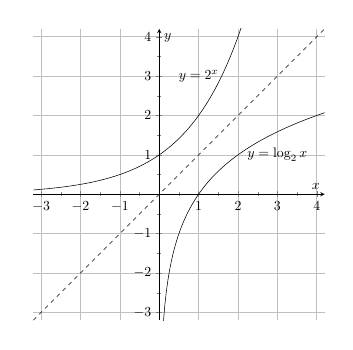
\begin{tikzpicture}[scale = 0.5]
                    \begin{axis}[
                        x=1.0cm,y=1.0cm,
                        axis lines=middle,
                        ymajorgrids=true,
                        xmajorgrids=true,
                        %xminorgrids=true,
                        %yminorgrids=true,
                        minor tick num=1,
                        xlabel = $x$,
                        ylabel =$y$,
                        xmin=-3.2,
                        xmax=4.2,
                        ymin=-3.2,
                        ymax=4.2,
                        xtick={-3.0,-2.0,...,4.0},
                        ytick={-3.0,-2.0,...,4.0},]
                        \draw [samples=100, domain=-3.2:4.2] plot(\x,{2^(\x)});
                        \draw [samples=100, domain=0.1:4.2] plot(\x,{log2(\x)});
                        \draw [dashed, samples=100, domain=-3.2:4.2] plot(\x,{\x});
                        \node at (1,3) {$y=2^x$};
                        \node at (3,1) {$y=\log_2 x$};
                    \end{axis}
                \end{tikzpicture}
        \end{wrapfigure}
        La funzione esponenziale è una funzione trascendente. Essa ha dominio $\R$ e codominio $]0;+\infty[$, e presenta un asintoto orizzontale a $0$. Di conseguenza non ha zeri di funzione. Se $a>1$ La funzione è strettamente crescente, mentre se $0<a<1$ la funzione è strettamente decrescente. 
    \subsection{La funzione logaritmo $y=\log_a x$}
        La funzione logaritmo è la funzione inversa della funzione esponenziale, di conseguenza ha dominio $]0;+\infty[$ e codominio $\R$. Presenta uno zero di funzione per $x=1$ e un asintoto verticale a $0$. Per $a>1$ è strettamente crescente, mentre per $0<a<1$ è strettamente decrescente. 

    \section{Grafica dedotta}
    \subsection{Trasformazioni geometriche}
    \subsubsection{Simmetria rispetto agli assi}
    \begin{wrapfigure}[3]{r}{0.3\textwidth}
        \centering
        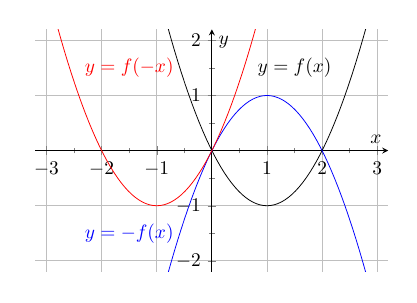
\begin{tikzpicture}[scale=0.7]
            \begin{axis}[
                x=1.0cm,y=1.0cm,
                axis lines=middle,
                ymajorgrids=true,
                xmajorgrids=true,
                %xminorgrids=true,
                %yminorgrids=true,
                minor tick num=1,
                xlabel = $x$,
                ylabel =$y$,
                xmin=-3.2,
                xmax=3.2,
                ymin=-2.2,
                ymax=2.2,
                xtick={-3.0,-2.0,...,3.0},
                ytick={-2.0,-1.0,...,2.0},]
                \draw [samples=100, domain=-3.2:3.2] plot(\x,{(\x)^2-2*\x});
                \draw [samples=100, domain=-3.2:3.2, color=blue] plot(\x,{-(\x)^2+2*\x});
                \draw [samples=100, domain=-3.2:3.2, color=red] plot(\x,{(\x)^2+2*\x});
                \node at (1.5,1.5) {$y=f(x)$};
                \node [color=blue] at (-1.5,-1.5) {$y=-f(x)$};
                \node [color=red] at (-1.5,1.5) {$y=f(-x)$};
            \end{axis}
        \end{tikzpicture}
        \caption*{$f(x)=x^2-2x$}
    \end{wrapfigure}
        Si consideri una funzione $y=f(x)$, è possibile tracciare i grafici delle simmetrie rispetto ai due asi cartesiani: in particolare $y=-f(x)$ è la simmetrica rispetto all'asse $x$, mentre $y=-f(x)$ è la simmetrica rispetto all'asse $y$.
    \subsubsection{Traslazione}
    \begin{wrapfigure}{r}{0.3\textwidth}
        \centering
        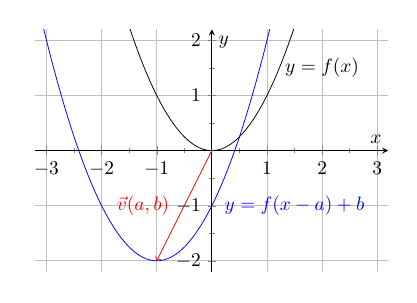
\begin{tikzpicture}[scale=0.7]
            \begin{axis}[
                x=1.0cm,y=1.0cm,
                axis lines=middle,
                ymajorgrids=true,
                xmajorgrids=true,
                %xminorgrids=true,
                %yminorgrids=true,
                minor tick num=1,
                xlabel = $x$,
                ylabel =$y$,
                xmin=-3.2,
                xmax=3.2,
                ymin=-2.2,
                ymax=2.2,
                xtick={-3.0,-2.0,...,3.0},
                ytick={-2.0,-1.0,...,2.0},]
                \draw [samples=100, domain=-3.2:3.2] plot(\x,{(\x)^2});
                \draw [samples=100, domain=-3.2:3.2, color=blue] plot(\x,{(\x)^2+2*\x-1});
                \draw [->, color=red] (0,0)--(-1,-2);
                \node at (2,1.5) {$y=f(x)$};
                \node [color=blue] at (1.5,-1) {$y=f(x-a)+b$};
                \node [color=red] at (-1.25,-1) {$\vec{v}(a,b)$};
            \end{axis}
        \end{tikzpicture}
    \end{wrapfigure}
        Data una funzione $y=f(x)$ e una traslazione di vettore $\vec{v}(a,b)$ ed equazione \[t:\left\lbrace\begin{array}{l}
            x'=x+a\\
            y'=y+b
        \end{array}\right.\]
        per ottenere l'equazione della funzione traslata è necesario ricavare la traslazione inversa e sostituire i valori di $x$ e $y$.
        \[t:\left\lbrace\begin{array}{l}
            x=x'-a\\
            y=y'-b
        \end{array}\right.\]
        \[y'-b=f(x'-a)\]
        \[y=f(x-a)+b\]
    \subsubsection{Dilatazione}
    \begin{wrapfigure}{r}{0.5\textwidth}
        \centering
        \begin{center}
            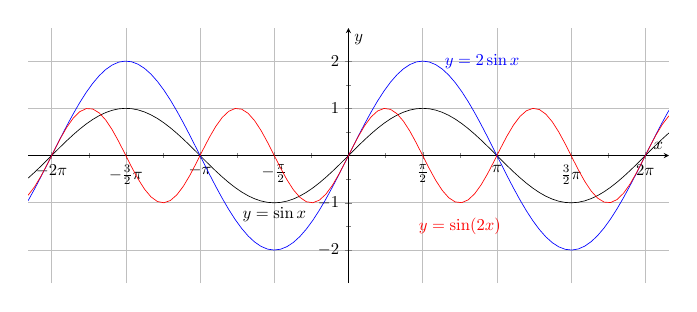
\begin{tikzpicture}[scale = 0.6]
                \begin{axis}[
                    x=1.0cm,y=1.0cm,
                    axis lines=middle,
                    ymajorgrids=true,
                    xmajorgrids=true,
                    %xminorgrids=true,
                    %yminorgrids=true,
                    minor tick num=1,
                    xlabel = $x$,
                    ylabel =$y$,
                    xmin=-2*pi-0.5,
                    xmax=2*pi+0.5,
                    ymin=-2.7,
                    ymax=2.7,
                    xtick={-2*pi,-3*pi/2,...,2*pi},
                    xticklabels={$-2\pi$, $-\frac{3}{2}\pi$, $-\pi$,$-\frac{\pi}{2}$,$0$,$\frac{\pi}{2}$,$\pi$, $\frac{3}{2}\pi$, $2\pi$},
                    ytick={-2.0,-1.0,...,2.0},]
                    \draw [samples=100, domain=-2*pi-0.5:2*pi+0.5] plot(\x,{sin(((\x))*180/pi)});
                    \draw [samples=100, domain=-2*pi-0.5:2*pi+0.5, color = blue] plot(\x,{2*sin(((\x))*180/pi)});
                    \draw [samples=100, domain=-2*pi-0.5:2*pi+0.5, color = red] plot(\x,{sin(((\x))*360/pi)});

                    \node at (-0.5*pi,-1.25) {$y=\sin x$};
                    \node[color=blue] at (0.9*pi,2){$y=2\sin x$};
                    \node[color=red] at (0.75*pi,-1.5){$y=\sin (2x)$};
                \end{axis}
            \end{tikzpicture}
        \end{center}
    \end{wrapfigure}
        Data una funzione $y=f(x)$ e una dilatazione di $a$ unità lungo l'asse $x$ e $b$ unità lungo l'asse $y$ 
        \[d:\left\lbrace
            \begin{array}{l}
                x'=ax\\
                y'=by
            \end{array}  \right.  
        \]
        per ottenere l'equazione della funzione dilatata è necesario ricavare la dilatazione inversa e sostituire i valori di $x$ e $y$.
        \[d:\left\lbrace
            \begin{array}{l}
                x=\dfrac{x'}{a}\\
                y=\dfrac{y'}{b}
            \end{array}  \right.  
        \]
        \[\frac{y}{b}=f\left(\frac{x}{a}\right)\]
        \[y=b\cdot f\left(\frac{x}{a}\right)\]
    \subsection{Funzione inversa}
        \begin{wrapfigure}[9]{r}{0.2\textwidth}
            \begin{center}
                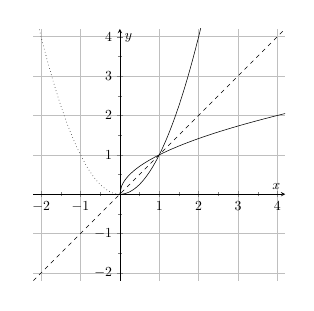
\begin{tikzpicture}[scale = 0.5]
                    \begin{axis}[
                        x=1.0cm,y=1.0cm,
                        axis lines=middle,
                        ymajorgrids=true,
                        xmajorgrids=true,
                        %xminorgrids=true,
                        %yminorgrids=true,
                        minor tick num=1,
                        xlabel = $x$,
                        ylabel =$y$,
                        xmin=-2.2,
                        xmax=4.2,
                        ymin=-2.2,
                        ymax=4.2,
                        xtick={-2.0,-1.0,...,4.0},
                        ytick={-2.0,-1.0,...,4.0},]
                        \draw [samples=100, domain=0:4.2] plot(\x,{sqrt(\x)});
                        \draw [samples=100, domain=0:4.2] plot(\x,{(\x)^2});
                        \draw [dotted, samples=100, domain=-2.2:0] plot(\x,{(\x)^2});
                        \draw [dashed, samples=100, domain=-2.2:4.2] plot(\x,{\x});
                    \end{axis}
                \end{tikzpicture}
            \end{center}
        \end{wrapfigure}
        Per poter tracciare il grafico di una funzione è necessario che una funzione sia biiettiva. Siccome ogni funzione è suriettiva nel proprio codominio, è necessario ridurne il dominio affinché sia anche iniettiva. Ad esemopio per poter rappresentare il grafico della funzione inversa di una funzione $y=x^2$ è necessario ridurne il dominio a $x\geq0$. A questo punto è possibile riscrivere la funzione nella forma $x=f^{-1}(y)$ ed effettuare un cambio di variabili arrivando quindi alla scrittura $y=f^{-1}(x)$. Per rappresentare il grafico della funzione inversa è sufficiente rappresentare la simmetrica della funzione di partenza rispetto alla bisettrice I-III quadrante, prestando attenzione al nuovo dominio ridotto.
    \subsection{Funzioni con valori assoluti}
    \begin{wrapfigure}{r}{0.3\textwidth}
        \centering
        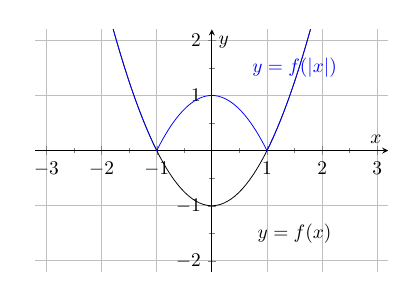
\begin{tikzpicture}[scale=0.7]
            \begin{axis}[
                x=1.0cm,y=1.0cm,
                axis lines=middle,
                ymajorgrids=true,
                xmajorgrids=true,
                %xminorgrids=true,
                %yminorgrids=true,
                minor tick num=1,
                xlabel = $x$,
                ylabel =$y$,
                xmin=-3.2,
                xmax=3.2,
                ymin=-2.2,
                ymax=2.2,
                xtick={-3.0,-2.0,...,3.0},
                ytick={-2.0,-1.0,...,2.0},]
                \draw [samples=100, domain=-3.2:3.2] plot(\x,{(\x)^2-1});
                \draw [samples=100, domain=-1:1, color=blue] plot(\x,{-(\x)^2+1});
                \draw [samples=100, domain=-3.2:-1, color=blue] plot(\x,{(\x)^2-1});
                \draw [samples=100, domain=1:3.2, color=blue] plot(\x,{(\x)^2-1});
                \node at (1.5,-1.5) {$y=f(x)$};
                \node [color=blue] at (1.5,1.5) {$y=f(|x|)$};
            \end{axis}
        \end{tikzpicture}
        \caption*{$f(x)=x^2-2x$}
    \end{wrapfigure}
    \subsubsection{$y=|f(x)|$}
        Recuperiamo la definizione di valore assoluto:
        \[|x|=\left\lbrace
            \begin{array}{ll}
                x &\text{se }x\geq 0\\
                -x&\text{se }x<0
            \end{array}\right. 
        \]
        Di conseguenza, sostituendo $f(x)$ ad $x$ nella definizione, si ottiene la definizione di $|f(x)|$
        \[|f(x)|=\left\lbrace
            \begin{array}{ll}
                f(x) &\text{se }f(x)\geq 0\\
                -f(x)&\text{se }f(x)<0
            \end{array}\right. 
        \]
        Questo significa che $|f(x)|$ coincide con $f(x)$ quando essa è maggiore di 0, e con la sua simmetrica rispetto all'asse $x$ quando $f(x)<0$.
    \subsubsection{$y=f(|x|)$}
        \begin{wrapfigure}[6]{r}{0.3\textwidth}
            \centering
            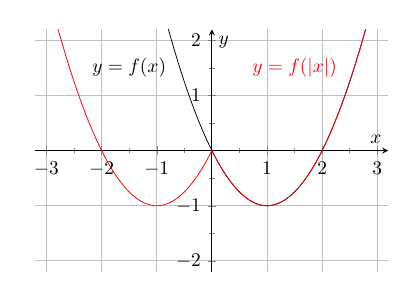
\begin{tikzpicture}[scale=0.7]
                \begin{axis}[
                    x=1.0cm,y=1.0cm,
                    axis lines=middle,
                    ymajorgrids=true,
                    xmajorgrids=true,
                    %xminorgrids=true,
                    %yminorgrids=true,
                    minor tick num=1,
                    xlabel = $x$,
                    ylabel =$y$,
                    xmin=-3.2,
                    xmax=3.2,
                    ymin=-2.2,
                    ymax=2.2,
                    xtick={-3.0,-2.0,...,3.0},
                    ytick={-2.0,-1.0,...,2.0},]
                    \draw [samples=100, domain=-3.2:3.2] plot(\x,{(\x)^2-2*\x});
                    \draw [samples=100, domain=-3.2:0, color=red] plot(\x,{(\x)^2+2*\x});
                    \draw [samples=100, domain=0:3.2, color=red] plot(\x,{(\x)^2-2*\x});
                    \node at (-1.5,1.5) {$y=f(x)$};
                    \node [color=red] at (1.5,1.5) {$y=f(|x|)$};
                \end{axis}
            \end{tikzpicture}
        \end{wrapfigure}
        Procedendo in modo analogo al punto precedente si ricava che
        \[f(|x|)=\left\lbrace
            \begin{array}{ll}
                f(x) &\text{se }x\geq 0\\
                f(-x)&\text{se }x<0
            \end{array}\right. 
        \]
        Di conseguenza la funzione è simmetrica rispetto all'asse delle $y$ in quanto coincide con $f(x)$ se $x\geq0$ e con $f(-x)$ (simmetrica di $f(x)$ rispetto all'asse $y$) quando $x<0$.
    \subsubsection{Funzioni con più valori assouti nidificati}
    \begin{wrapfigure}{r}{0.3\textwidth}
        \centering
        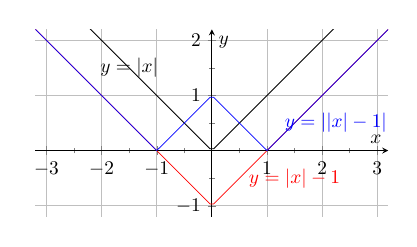
\begin{tikzpicture}[scale=0.7]
            \begin{axis}[
                x=1.0cm,y=1.0cm,
                axis lines=middle,
                ymajorgrids=true,
                xmajorgrids=true,
                %xminorgrids=true,
                %yminorgrids=true,
                minor tick num=1,
                xlabel = $x$,
                ylabel =$y$,
                xmin=-3.2,
                xmax=3.2,
                ymin=-1.2,
                ymax=2.2,
                xtick={-3.0,-2.0,...,3.0},
                ytick={-1.0,-0.0,...,2.0},]
                \draw [samples=100, domain=-3.2:3.2] plot(\x,{abs(\x)});
                \draw [samples=100, domain=-3.2:3.2, color=red] plot(\x,{abs(\x)-1});
                \draw [samples=100, domain=-3.2:3.2, color=blue] plot(\x,{abs(abs(\x)-1)});
                \node at (-1.5,1.5) {$y=|x|$};
                \node [color=red] at (1.5,-0.5) {$y=|x|-1$};
                \node [color=blue] at (2.25,0.5) {$y=||x|-1|$};
            \end{axis}
        \end{tikzpicture}
    \end{wrapfigure}
        In questo caso è sufficiente procedere per gradi: consideriamo ad esempio la funzione $y=||x|-1|$. Il metodo migliore è quindi rappresentare prima la funzione $y=|x|$, successivamente traslarla verso il basso di 1 unità ($y=|x|-1$) e poi rappresentare anche il modulo più esterno effettuando al simmetria rispetto all'asse x della regione negativa. 
    \subsubsection{Funzioni con più valori assoluti in sequenza}
        Qui la situazione si complica, perché è necessario studiare tutti gli intervalli di positività che i diversi argomenti dei valori assoluti possono assumere. Consideriamo ad esempio la funzione $y=|x-1|+|2x+4|$.
        Prima di tutto bisogna trovare per quali valori di $x$ l'argomento di ogni valore assoluto assume valori non negativi.
        \[x-1\geq0 ~~~~~~x\geq 1\]
        \[2x+4\geq0~~~~~~x\geq -2 \]
        A questo punto rappresentiamo gli intervalli trovati.
        
        \begin{figure}[h]
            \centering
            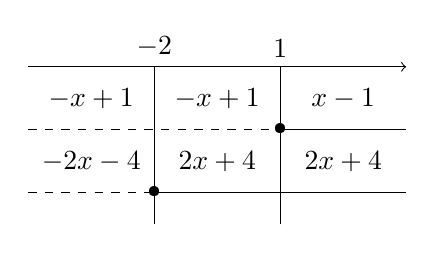
\begin{tikzpicture}[scale=0.8]
                \draw [->] (0,3)--(6,3);
                \draw (2,0.5)--(2,3) node[above]{$-2$};
                \draw (4,0.5)--(4,3) node[above]{$1$};
                \draw [dashed] (0,2)--(4,2);
                \draw (4,2)--(6,2);
                \node at (4,2) {\textbullet};
                \draw [dashed] (0,1)--(2,1);
                \draw (2,1)--(6,1);
                \node at (2,1) {\textbullet};
    
                \node at (1,2.5){$-x+1$};
                \node at (3,2.5){$-x+1$};
                \node at (5,2.5){$x-1$};
    
                \node at (1,1.5){$-2x-4$};
                \node at (3,1.5){$2x+4$};
                \node at (5,1.5){$2x+4$};
            \end{tikzpicture}
        \end{figure}

        A questo punto possiamo usare lo schema appena trovato per ricostruire la funzione come definita a tratti:
        \begin{wrapfigure}[6]{r}{0.3\textwidth}
            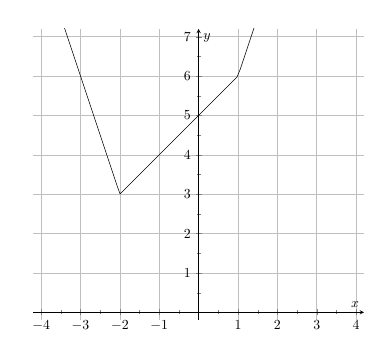
\begin{tikzpicture}[scale=0.5]
                \begin{axis}[
                    x=1.0cm,y=1.0cm,
                    axis lines=middle,
                    ymajorgrids=true,
                    xmajorgrids=true,
                    %xminorgrids=true,
                    %yminorgrids=true,
                    minor tick num=1,
                    xlabel = $x$,
                    ylabel =$y$,
                    xmin=-4.2,
                    xmax=4.2,
                    ymin=-0.2,
                    ymax=7.2,
                    xtick={-4.0,-3.0,...,4.0},
                    ytick={-0.0,-1.0,...,7.0},]
                    \draw [samples=100, domain=-4.2:4.2] plot(\x,{abs(\x-1)+abs(2*\x+4)});
                \end{axis}
            \end{tikzpicture}
        \end{wrapfigure}
        \[
        y=\left\lbrace\begin{array}{ll}
            (-x+1)+(-2x-4) &\text{se }x<-2\\
            (-x+1)+(2x+4) &\text{se }-2\leq x<1\\
            (x-1)+(2x+4) &\text{se }x\geq 1
        \end{array}\right.    
        \]
        \[
        y=\left\lbrace\begin{array}{ll}
            -3x-3 &\text{se }x<-2\\
            x+5 &\text{se }-2\leq x<1\\
            3x+3 &\text{se }x\geq 1
        \end{array}\right.    
        \]
    \subsection{Reciproco di una funzione}
        \begin{ex*}
            Tracciare il grafico di $y=\frac{1}{x^2-1}$
        \end{ex*}
            Cominciamo con il tracciare il grafico di $y=x^2-1$. Si tratta di una parabola di vertice $V(0,-1)$.
        \begin{figure}[h]
            \centering
            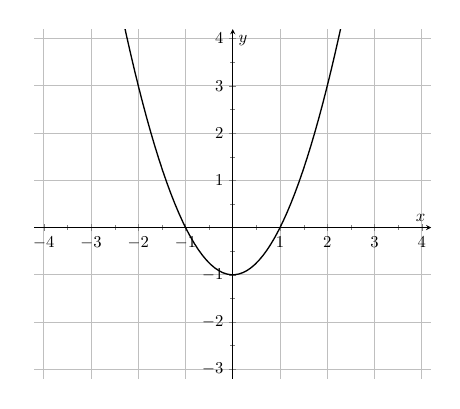
\begin{tikzpicture}[scale=0.6]
                \begin{axis}[
                    x=1.0cm,y=1.0cm,
                    axis lines=middle,
                    ymajorgrids=true,
                    xmajorgrids=true,
                    %xminorgrids=true,
                    %yminorgrids=true,
                    minor tick num=1,
                    xlabel = $x$,
                    ylabel =$y$,
                    xmin=-4.2,
                    xmax=4.2,
                    ymin=-3.2,
                    ymax=4.2,
                    xtick={-4.0,-3.0,...,4.0},
                    ytick={-0.0,-1.0,...,7.0},]
                    \draw [samples=100, domain=-4.2:4.2, thick] plot(\x,{(\x)^2-1});
                \end{axis}
            \end{tikzpicture}
        \end{figure}

        A questo punto procediamo con l'analisi del dominio: sappiamo che il dominio di una fratta si ricava ponendo il denominatore diverso da $0$, quindi il domino di $\frac{1}{f(x)}$ si ottiene trovando dove $f(x)\neq0$
        \[D: x^2-1\neq 0\]
        \[(x-1)(x+1)\neq 0\]
        \[x\neq \pm 1\]
        \[D: ]-\infty;-1[\cup]-1;1[\cup]1;+\infty[\]
        In particolare dove $f(x)=0$, $\frac{1}{f(x)}$ presenta degli asintoti verticali. Il prossimo passo è studiare i punti di intersezione delle due funzioni. Siccome $f(x)=\frac{1}{f(x)}$ se $f(x)=\pm 1$, le due funzioni si intersecano solo dove intersecano la retta $y=1$ o la retta $y=-1$. Rappresentiamo quanto ottenuto.
        \begin{figure}[h]
            \centering
            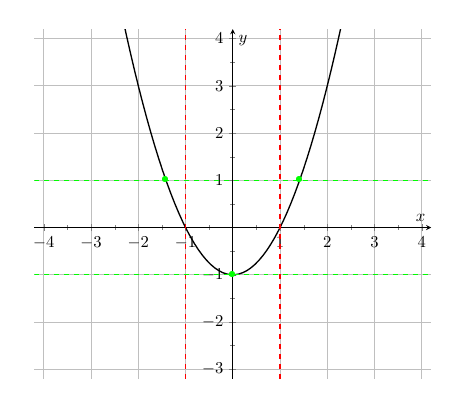
\begin{tikzpicture}[scale=0.6]
                \begin{axis}[
                    x=1.0cm,y=1.0cm,
                    axis lines=middle,
                    ymajorgrids=true,
                    xmajorgrids=true,
                    %xminorgrids=true,
                    %yminorgrids=true,
                    minor tick num=1,
                    xlabel = $x$,
                    ylabel =$y$,
                    xmin=-4.2,
                    xmax=4.2,
                    ymin=-3.2,
                    ymax=4.2,
                    xtick={-4.0,-3.0,...,4.0},
                    ytick={-0.0,-1.0,...,7.0},]
                    \draw [samples=100, domain=-4.2:4.2, thick] plot(\x,{(\x)^2-1});
                    \draw [dashed, color=red, thick] (-1,-3.2)--(-1,4.2);
                    \draw [dashed, color=red, thick] (1,-3.2)--(1,4.2);

                    \draw [dashed, color=green, thick] (-4.2,1)--(4.2,1);
                    \draw [dashed, color=green, thick] (-4.2,-1)--(4.2,-1);
                    \node [color=green] at (0,-1){\textbullet};
                    \node [color=green] at (-1.41421,1){\textbullet};
                    \node [color=green] at (1.41421,1){\textbullet};
                \end{axis}
            \end{tikzpicture}
        \end{figure}
        A questo punto rimane solo un passaggio prima di poter rappresentare la funzione: studiare i limiti negli intorni degli estremi del dominio. 
        \[\renewcommand{\arraystretch}{1.8}\begin{array}{lllll}
            x \rightarrow -\infty &~~~& f(x)\rightarrow +\infty &~~~& \dfrac{1}{f(x)}\rightarrow 0^+\\
            x \rightarrow -1^- &~~~& f(x)\rightarrow 0^+ &~~~& \dfrac{1}{f(x)}\rightarrow +\infty\\
            x \rightarrow -1^+ &~~~& f(x)\rightarrow 0^- &~~~& \dfrac{1}{f(x)}\rightarrow -\infty\\
            x \rightarrow 1^- &~~~& f(x)\rightarrow 0^- &~~~& \dfrac{1}{f(x)}\rightarrow -\infty\\
            x \rightarrow 1^+ &~~~& f(x)\rightarrow 0^+ &~~~& \dfrac{1}{f(x)}\rightarrow +\infty\\
            x \rightarrow +\infty &~~~& f(x)\rightarrow +\infty &~~~& \dfrac{1}{f(x)}\rightarrow 0^+\\
        \end{array}\]
        \begin{figure}[h]
            \centering
            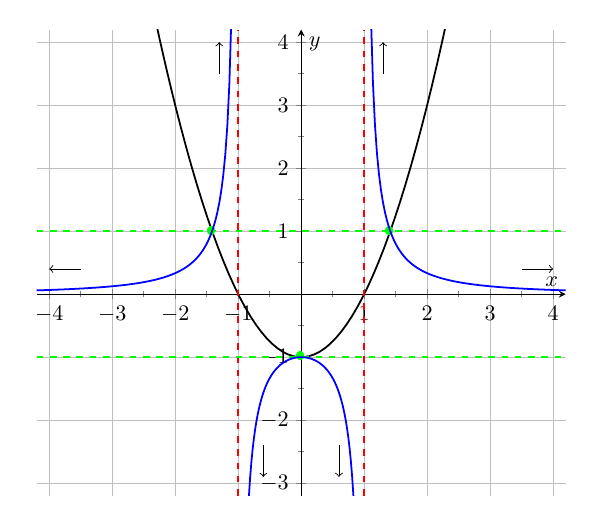
\begin{tikzpicture}[scale=0.8]
                \begin{axis}[
                    x=1.0cm,y=1.0cm,
                    axis lines=middle,
                    ymajorgrids=true,
                    xmajorgrids=true,
                    %xminorgrids=true,
                    %yminorgrids=true,
                    minor tick num=1,
                    xlabel = $x$,
                    ylabel =$y$,
                    xmin=-4.2,
                    xmax=4.2,
                    ymin=-3.2,
                    ymax=4.2,
                    xtick={-4.0,-3.0,...,4.0},
                    ytick={-0.0,-1.0,...,7.0},]
                    \draw [samples=100, domain=-4.2:4.2, thick] plot(\x,{(\x)^2-1});
                    \draw [dashed, color=red, thick] (-1,-3.2)--(-1,4.2);
                    \draw [dashed, color=red, thick] (1,-3.2)--(1,4.2);

                    \draw [dashed, color=green, thick] (-4.2,1)--(4.2,1);
                    \draw [dashed, color=green, thick] (-4.2,-1)--(4.2,-1);
                    \node [color=green] at (0,-1){\textbullet};
                    \node [color=green] at (-1.41421,1){\textbullet};
                    \node [color=green] at (1.41421,1){\textbullet};

                    \draw [->] (-3.5,0.4)--(-4,0.4);
                    \draw [->] (-1.3,3.5)--(-1.3,4);
                    \draw [->] (-0.6,-2.4)--(-0.6,-2.9);
                    \draw [->] (0.6,-2.4)--(0.6,-2.9);
                    \draw [->] (1.3,3.5)--(1.3,4);
                    \draw [->] (3.5,0.4)--(4,0.4);

                    \draw [samples=100, domain=-4.2:-1.01, thick, color=blue] plot(\x,{1/((\x)^2-1)});
                    \draw [samples=100, domain=-0.99:0.99, thick, color=blue] plot(\x,{1/((\x)^2-1)});
                    \draw [samples=100, domain=1.01:4.2, thick, color=blue] plot(\x,{1/((\x)^2-1)});
                \end{axis}
            \end{tikzpicture}
        \end{figure} \newpage
    \subsection{Quadrato di una funzione}   
        \begin{ex*}
            Tracciare il grafico di $y=\sin^2x$
        \end{ex*}
        Cominciamo con il tracciare il grafico della funzione elementare $y=\sin x$\\
        \begin{figure}[h]
            \centering
            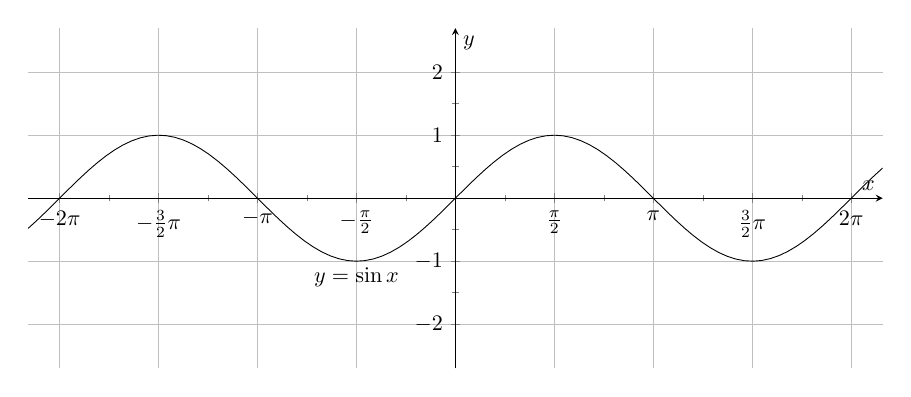
\begin{tikzpicture}[scale = 0.8]
                \begin{axis}[
                    x=1.0cm,y=1.0cm,
                    axis lines=middle,
                    ymajorgrids=true,
                    xmajorgrids=true,
                    %xminorgrids=true,
                    %yminorgrids=true,
                    minor tick num=1,
                    xlabel = $x$,
                    ylabel =$y$,
                    xmin=-2*pi-0.5,
                    xmax=2*pi+0.5,
                    ymin=-2.7,
                    ymax=2.7,
                    xtick={-2*pi,-3*pi/2,...,2*pi},
                    xticklabels={$-2\pi$, $-\frac{3}{2}\pi$, $-\pi$,$-\frac{\pi}{2}$,$0$,$\frac{\pi}{2}$,$\pi$, $\frac{3}{2}\pi$, $2\pi$},
                    ytick={-2.0,-1.0,...,2.0},]
                    \draw [samples=100, domain=-2*pi-0.5:2*pi+0.5] plot(\x,{sin(((\x))*180/pi)});
                    %\draw [samples=100, domain=-2*pi-0.5:2*pi+0.5, color = blue] plot(\x,{2*sin(((\x))*180/pi)});

                    \node at (-0.5*pi,-1.25) {$y=\sin x$};
                    %\node[color=blue] at (0.9*pi,2){$y=2\sin x$};
                \end{axis}
            \end{tikzpicture}
        \end{figure}

        Per qanto riguarda il dominio, esso rimane invariato. Siccome il dominio della funzione di partenza $f(x)$ è $\R$, il dominio di $f^2(x)$ rimane $\R$. Siccome il quadrato di un numero reale è sempre non negatico, procediamo con il rappresentare $|f(x)|$. Essa inoltre interseca $f^2(x)$ lungo le rette $y=0$ e $y=1$ .\\
        \begin{figure}[h]
            \centering
            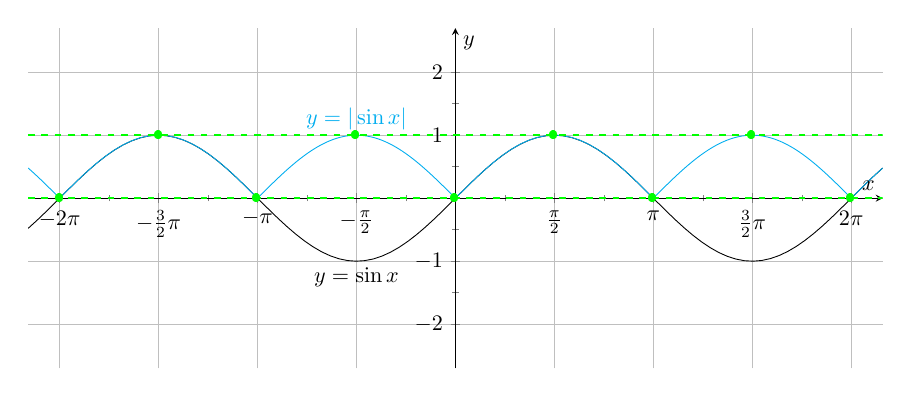
\begin{tikzpicture}[scale = 0.8]
                \begin{axis}[
                    x=1.0cm,y=1.0cm,
                    axis lines=middle,
                    ymajorgrids=true,
                    xmajorgrids=true,
                    %xminorgrids=true,
                    %yminorgrids=true,
                    minor tick num=1,
                    xlabel = $x$,
                    ylabel =$y$,
                    xmin=-2*pi-0.5,
                    xmax=2*pi+0.5,
                    ymin=-2.7,
                    ymax=2.7,
                    xtick={-2*pi,-3*pi/2,...,2*pi},
                    xticklabels={$-2\pi$, $-\frac{3}{2}\pi$, $-\pi$,$-\frac{\pi}{2}$,$0$,$\frac{\pi}{2}$,$\pi$, $\frac{3}{2}\pi$, $2\pi$},
                    ytick={-2.0,-1.0,...,2.0},]
                    \draw [samples=100, domain=-2*pi-0.5:2*pi+0.5] plot(\x,{sin(((\x))*180/pi)});
                    \draw [samples=100, domain=-2*pi-0.5:-2*pi, color = cyan, smooth] plot(\x,{-sin(((\x))*180/pi)});
                        \draw [samples=100, domain=-2*pi:-pi, color = cyan, smooth] plot(\x,{sin(((\x))*180/pi)});
                        \draw [samples=100, domain=-pi:0, color = cyan, smooth] plot(\x,{-sin(((\x))*180/pi)});
                        \draw [samples=100, domain=0:pi, color = cyan, smooth] plot(\x,{sin(((\x))*180/pi)});
                        \draw [samples=100, domain=pi:2*pi, color = cyan, smooth] plot(\x,{-sin(((\x))*180/pi)});
                        \draw [samples=100, domain=2*pi:2*pi+0.5, color = cyan, smooth] plot(\x,{sin(((\x))*180/pi)});
                    %\draw [samples=100, domain=-2*pi-0.5:2*pi+0.5, color = blue] plot(\x,{(sin(((\x))*180/pi))^2});

                    \node at (-0.5*pi,-1.25) {$y=\sin x$};
                    \node[color=cyan] at (-0.5*pi,1.25){$y=|\sin x|$};
                    %\node[color=blue] at (0.9*pi,2){$y=\sin^2 x$};

                    \draw [dashed, color=green, thick] (-2*pi-0.5,1)--(2*pi+0.5,1);
                    \node [color=green] at (-1.5*pi,1){\textbullet};
                    \node [color=green] at (-0.5*pi,1){\textbullet};
                    \node [color=green] at (1.5*pi,1){\textbullet};
                    \node [color=green] at (0.5*pi,1){\textbullet};

                    \draw [dashed, color=green, thick] (-2*pi-0.5,0)--(2*pi+0.5,0);
                    \node [color=green] at (-2*pi,0){\textbullet};
                    \node [color=green] at (-pi,0){\textbullet};
                    \node [color=green] at (0,0){\textbullet};
                    \node [color=green] at (pi,0){\textbullet};
                    \node [color=green] at (2*pi,0){\textbullet};
                \end{axis}
            \end{tikzpicture}
        \end{figure}

        L'ultima cosa da tenere in considerazione è che se $0<|f(x)|<1$, $f^2(x)<|f(x)|$; mentre se $|f(x)|>1$, $f^2(x)>|f(x)|$. A questo punto abbiamo tutte le informazioni necessarie per tracciare il grafico di $f^2(x)$.

        \begin{figure}[h]
            \centering
            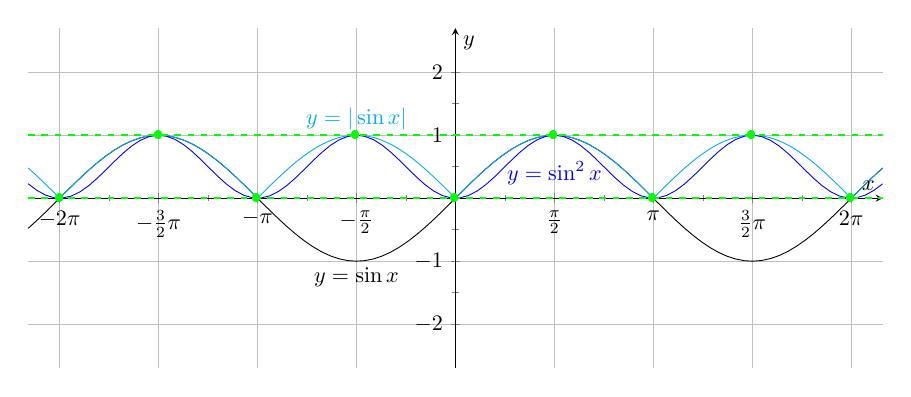
\begin{tikzpicture}[scale = 0.8]
                \begin{axis}[
                    x=1.0cm,y=1.0cm,
                    axis lines=middle,
                    ymajorgrids=true,
                    xmajorgrids=true,
                    %xminorgrids=true,
                    %yminorgrids=true,
                    minor tick num=1,
                    xlabel = $x$,
                    ylabel =$y$,
                    xmin=-2*pi-0.5,
                    xmax=2*pi+0.5,
                    ymin=-2.7,
                    ymax=2.7,
                    xtick={-2*pi,-3*pi/2,...,2*pi},
                    xticklabels={$-2\pi$, $-\frac{3}{2}\pi$, $-\pi$,$-\frac{\pi}{2}$,$0$,$\frac{\pi}{2}$,$\pi$, $\frac{3}{2}\pi$, $2\pi$},
                    ytick={-2.0,-1.0,...,2.0},]
                    \draw [samples=100, domain=-2*pi-0.5:2*pi+0.5] plot(\x,{sin(((\x))*180/pi)});
                    \draw [samples=100, domain=-2*pi-0.5:-2*pi, color = cyan, smooth] plot(\x,{-sin(((\x))*180/pi)});
                        \draw [samples=100, domain=-2*pi:-pi, color = cyan, smooth] plot(\x,{sin(((\x))*180/pi)});
                        \draw [samples=100, domain=-pi:0, color = cyan, smooth] plot(\x,{-sin(((\x))*180/pi)});
                        \draw [samples=100, domain=0:pi, color = cyan, smooth] plot(\x,{sin(((\x))*180/pi)});
                        \draw [samples=100, domain=pi:2*pi, color = cyan, smooth] plot(\x,{-sin(((\x))*180/pi)});
                        \draw [samples=100, domain=2*pi:2*pi+0.5, color = cyan, smooth] plot(\x,{sin(((\x))*180/pi)});
                    \draw [samples=100, domain=-2*pi-0.5:2*pi+0.5, color = blue] plot(\x,{(sin(((\x))*180/pi))^2});

                    \node at (-0.5*pi,-1.25) {$y=\sin x$};
                    \node[color=cyan] at (-0.5*pi,1.25){$y=|\sin x|$};
                    \node[color=blue] at (0.5*pi,0.4){$y=\sin^2 x$};

                    \draw [dashed, color=green, thick] (-2*pi-0.5,1)--(2*pi+0.5,1);
                    \node [color=green] at (-1.5*pi,1){\textbullet};
                    \node [color=green] at (-0.5*pi,1){\textbullet};
                    \node [color=green] at (1.5*pi,1){\textbullet};
                    \node [color=green] at (0.5*pi,1){\textbullet};

                    \draw [dashed, color=green, thick] (-2*pi-0.5,0)--(2*pi+0.5,0);
                    \node [color=green] at (-2*pi,0){\textbullet};
                    \node [color=green] at (-pi,0){\textbullet};
                    \node [color=green] at (0,0){\textbullet};
                    \node [color=green] at (pi,0){\textbullet};
                    \node [color=green] at (2*pi,0){\textbullet};
                \end{axis}
            \end{tikzpicture}
        \end{figure}
    \subsection{Radice di una funzione}
        \begin{ex*}
            Tracciare il grafico di $y=\sqrt{\tg x}$
        \end{ex*}
        Cominciamo con il tracciare il grafico della funzione elementare $y=\tg x$. Siccome il domino della funzione irrazionale si ottiene ponendo il radicando $\geq 0$, il dominio della funzione $y=\sqrt{\tg x}$ è $D: [k\pi; \frac{\pi}{2}+k\pi]$ con $k\in \Z$. A questo punto, analogamente a quanto fatto precedentemente, sappiamo che le funzioni $y=f(x)$ e $y=\sqrt{f(x)}$ si intersecano per $f(x)=0$ e $f(x)=1$. Sappiamo inoltre che se se $0<f(x)<1$, $\sqrt{f(x)}>f(x)$; mentre se $f(x)>1$, $\sqrt{f(x)}<f(x)$. A questo punto abbiamo tutte le informazioni necessarie per tracciare il grafico di $\sqrt{f(x)}$.
        \begin{figure}[h]
            \centering
            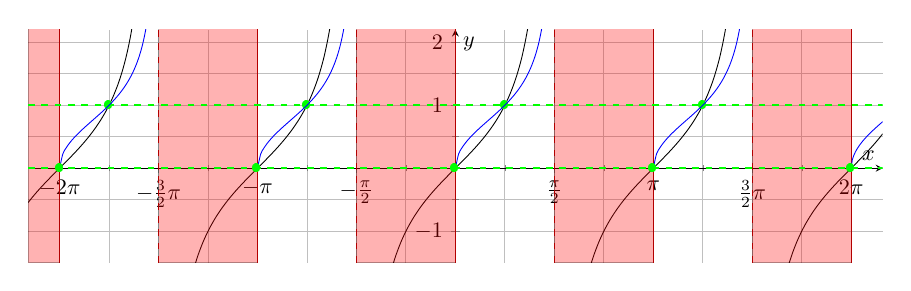
\begin{tikzpicture}[scale = 0.8]
                \begin{axis}[
                    x=1.0cm,y=1.0cm,
                    axis lines=middle,
                    ymajorgrids=true,
                    xmajorgrids=true,
                    xminorgrids=true,
                    yminorgrids=true,
                    minor tick num=1,
                    xlabel = $x$,
                    ylabel =$y$,
                    xmin=-2*pi-0.5,
                    xmax=2*pi+0.5,
                    ymin=-1.5,
                    ymax=2.2,
                    xtick={-2*pi,-3*pi/2,...,2*pi},
                    xticklabels={$-2\pi$, $-\frac{3}{2}\pi$, $-\pi$,$-\frac{\pi}{2}$,$0$,$\frac{\pi}{2}$,$\pi$, $\frac{3}{2}\pi$, $2\pi$},
                    ytick={-1.0,0.0,...,2.0},]
                    \draw[smooth,samples=30,domain=-0.5*pi+0.1:+0.5*pi-0.1] plot(\x,{tan(((\x))*180/pi)});
                    \draw[smooth,samples=30,domain=-1.5*pi+0.1:-0.5*pi-0.1] plot(\x,{tan(((\x))*180/pi)});
                    \draw[smooth,samples=30,domain=-2.0*pi-0.5:-1.5*pi-0.1] plot(\x,{tan(((\x))*180/pi)});
                    \draw[smooth,samples=30,domain=0.5*pi+0.1:1.5*pi-0.1] plot(\x,{tan(((\x))*180/pi)});
                    \draw[smooth,samples=30,domain=1.5*pi+0.1:2.0*pi+0.5] plot(\x,{tan(((\x))*180/pi)});

                    \draw[dashed, color=red] (0.5*pi,-1.5)--(0.5*pi,2.5);
                    \draw[dashed, color=red] (-0.5*pi,-1.5)--(-0.5*pi,2.5);
                    \draw[dashed, color=red] (1.5*pi,-1.5)--(1.5*pi,2.5);
                    \draw[dashed, color=red] (-1.5*pi,-1.5)--(-1.5*pi,2.5);

                    \draw[color=red] (pi,-1.5)--(pi,2.5);
                    \draw[color=red] (-pi,-1.5)--(-pi,2.5);
                    \draw[color=red] (2*pi,-1.5)--(2*pi,2.5);
                    \draw[color=red] (-2*pi,-1.5)--(-2*pi,2.5);%
                    \draw[color=red] (0,-1.5)--(0,2.5);

                    \draw[fill=red, opacity=0.3] (-2*pi,-1.5)--(-2*pi,2.5)--(-2*pi-0.5,2.5)--(-2*pi-0.5,-1.5)--cycle;
                    \draw[fill=red, opacity=0.3] (-1.5*pi,-1.5)--(-1.5*pi,2.5)--(-pi,2.5)--(-pi,-1.5)--cycle;
                    \draw[fill=red, opacity=0.3] (-0.5*pi,-1.5)--(-0.5*pi,2.5)--(0,2.5)--(0,-1.5)--cycle;
                    \draw[fill=red, opacity=0.3] (0.5*pi,-1.5)--(0.5*pi,2.5)--(pi,2.5)--(pi,-1.5)--cycle;
                    \draw[fill=red, opacity=0.3] (1.5*pi,-1.5)--(1.5*pi,2.5)--(2*pi,2.5)--(2*pi,-1.5)--cycle;

                    \draw [dashed, color=green, thick] (-2*pi-0.5,1)--(2*pi+0.5,1);
                    \node [color=green] at (-1.75*pi,1){\textbullet};
                    \node [color=green] at (-0.75*pi,1){\textbullet};
                    \node [color=green] at (1.25*pi,1){\textbullet};
                    \node [color=green] at (0.25*pi,1){\textbullet};
                    
                    \draw[color=blue, smooth,samples=30,domain=0:+0.5*pi-0.1] plot(\x,{sqrt(tan(((\x))*180/pi))});
                    \draw[color=blue, smooth,samples=30,domain=-pi:-0.5*pi-0.1] plot(\x,{sqrt(tan(((\x))*180/pi))});
                    \draw[color=blue, smooth,samples=30,domain=-2.0*pi:-1.5*pi-0.1] plot(\x,{sqrt(tan(((\x))*180/pi))});
                    \draw[color=blue, smooth,samples=30,domain=pi:1.5*pi-0.1] plot(\x,{sqrt(tan(((\x))*180/pi))});
                    \draw[color=blue, smooth,samples=30,domain=2.0*pi:2.0*pi+0.5] plot(\x,{sqrt(tan(((\x))*180/pi))});
                    
                    \draw [dashed, color=green, thick] (-2*pi-0.5,0)--(2*pi+0.5,0);
                    \node [color=green] at (-2*pi,0){\textbullet};
                    \node [color=green] at (-pi,0){\textbullet};
                    \node [color=green] at (0,0){\textbullet};
                    \node [color=green] at (pi,0){\textbullet};
                    \node [color=green] at (2*pi,0){\textbullet};
                \end{axis}
            \end{tikzpicture}
        \end{figure}

        \subsection{Esponenziale di una funzione}
            \begin{ex*}
                Tracciare il grafico di $y=e^{\frac{x-2}{x-1}}$
            \end{ex*}
            Per prima cosa tracciamo il grafico di $y=\frac{x-2}{x-1}$. Questa funzione ha un asintoto orizzontale per $y=1$ e un asintoto verticale per $x=1$.
            \begin{figure}[ht]
                \centering
                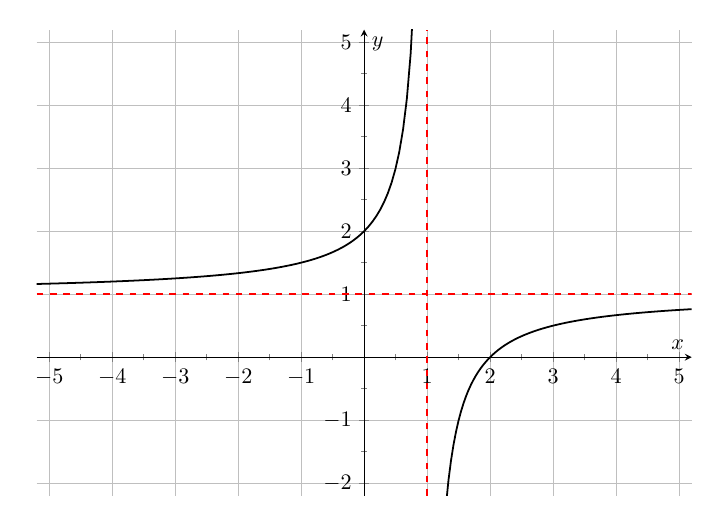
\begin{tikzpicture}[scale=0.8]
                    \begin{axis}[
                        x=1.0cm,y=1.0cm,
                        axis lines=middle,
                        ymajorgrids=true,
                        xmajorgrids=true,
                        %xminorgrids=true,
                        %yminorgrids=true,
                        minor tick num=1,
                        xlabel = $x$,
                        ylabel =$y$,
                        xmin=-5.2,
                        xmax=5.2,
                        ymin=-2.2,
                        ymax=5.2,
                        xtick={-5.0,-4.0,...,5.0},
                        ytick={-2.0,-1.0,...,5.0},]
                        \draw [samples=100, domain=-5.2:0.8, thick] plot(\x,{(\x-2)/(\x-1)});
                        \draw [samples=100, domain=1.3:5.2, thick] plot(\x,{(\x-2)/(\x-1)});
                        \draw [dashed, color=red, thick] (-5.2,1)--(5.2,1);
                        \draw [dashed, color=red, thick] (1,-2.2)--(1,5.2);
                        
                    \end{axis}
                \end{tikzpicture}
            \end{figure}

            Siccome il dominio di $e^{f(x)}$ coincide con il dominio di $f(x)$, l'asintoto verticale si conserva. L'asintoto orizzontale invece si sposta passando da $y=1$ a $y=e^1$. Inoltre, dove la funzione va a 0, sappiamo che $e^0=1$, quindi la nuova funzione passerà per 1. L'ultimo passo prima di poter rappresentare la funzione consiste nello studiarne i limiti agli estremi del dominio.
            \[\renewcommand{\arraystretch}{1.8}\begin{array}{lllll}
                x \rightarrow -\infty &~~~& f(x)\rightarrow 1^+ &~~~& e^{f(x)}\rightarrow e^+\\
                x \rightarrow 1^- &~~~& f(x)\rightarrow +\infty &~~~& e^{f(x)}\rightarrow +\infty\\
                x \rightarrow 1^+ &~~~& f(x)\rightarrow -\infty &~~~& e^{f(x)}\rightarrow 0^+\\
                x \rightarrow +\infty &~~~& f(x)\rightarrow 1^- &~~~& e^{f(x)}\rightarrow e^-\\
            \end{array}\]
        \begin{figure}[ht]
            \centering
            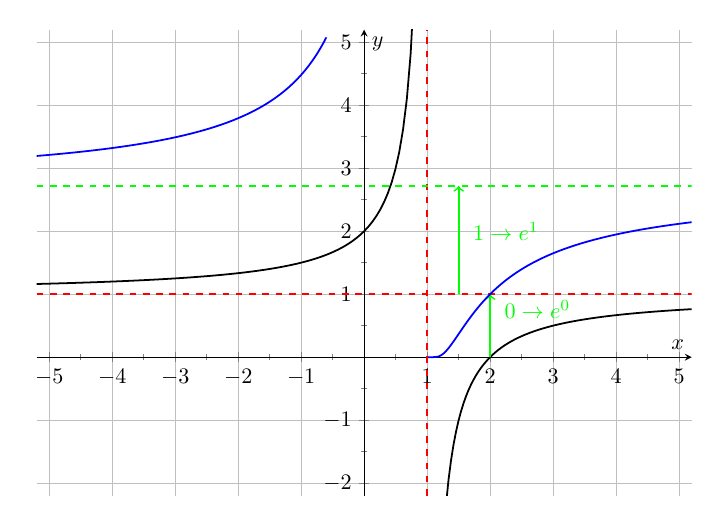
\begin{tikzpicture}[scale=0.8]
                \begin{axis}[
                    x=1.0cm,y=1.0cm,
                    axis lines=middle,
                    ymajorgrids=true,
                    xmajorgrids=true,
                    %xminorgrids=true,
                    %yminorgrids=true,
                    minor tick num=1,
                    xlabel = $x$,
                    ylabel =$y$,
                    xmin=-5.2,
                    xmax=5.2,
                    ymin=-2.2,
                    ymax=5.2,
                    xtick={-5.0,-4.0,...,5.0},
                    ytick={-2.0,-1.0,...,5.0},]
                    \draw [samples=100, domain=-5.2:0.8, thick] plot(\x,{(\x-2)/(\x-1)});
                    \draw [samples=100, domain=1.3:5.2, thick] plot(\x,{(\x-2)/(\x-1)});
                    \draw [dashed, color=red, thick] (-5.2,1)--(5.2,1);
                    \draw [dashed, color=red, thick] (1,-2.2)--(1,5.2);

                    \draw [dashed, color=green, thick] (-5.2,e)--(5.2,e);

                    \coordinate (A) at (1.5,1);
                    \coordinate (A') at (1.5,e);
                    \draw[->, thick, color=green] (A)--(A');
                    \node[color=green] at (2.25,2) {$1\rightarrow e^1$};

                    \coordinate (Z) at (2,0);
                    \coordinate (Z') at (2,1);
                    \draw[->, thick, color=green] (Z)--(Z');
                    \node[color=green] at (2.75,0.75) {$0\rightarrow e^0$};

                    %\draw [->] (-3.5,0.4)--(-4,0.4);
                    %\draw [->] (-1.3,3.5)--(-1.3,4);
                    %\draw [->] (-0.6,-2.4)--(-0.6,-2.9);
                    %\draw [->] (0.6,-2.4)--(0.6,-2.9);
                    %\draw [->] (1.3,3.5)--(1.3,4);
                    %\draw [->] (3.5,0.4)--(4,0.4);

                    \draw [samples=100, domain=-5.2:-0.6, thick, color=blue] plot(\x,{e^((\x-2)/(\x-1))});
                    \draw [samples=100, domain=1.01:5.2, thick, color=blue] plot(\x,{e^((\x-2)/(\x-1))});
                    
                \end{axis}
            \end{tikzpicture}
        \end{figure}

    \subsection{Logaritmo di una funzione}
        \begin{ex*}
            Tracciare il grafico di $y=\ln{\frac{x-2}{x-1}}$
        \end{ex*}
        Per prima cosa tracciamo il grafico di $y=\frac{x-2}{x-1}$. Questa funzione ha un asintoto orizzontale per $y=1$ e un asintoto verticale per $x=1$. Sicome la funzione $y=\ln f(x)$ ha dominio $f(x)> 0$. Di conseguenza, risolvendo la disequazione $\frac{x-2}{x-1}> 0$ otteniamo l'intervallo $D: ]-\infty;1[\cup]2;+\infty[$. L'asintoto orizzontale si sposta passando da $y=1$ a $y=\ln 1=0$. L'ultimo passo prima di poter rappresentare la funzione consiste nello studiarne i limiti agli estremi del dominio.
        \[\renewcommand{\arraystretch}{1.8}\begin{array}{lllll}
            x \rightarrow -\infty &~~~& f(x)\rightarrow 1^+ &~~~& \ln{f(x)}\rightarrow 0^+\\
            x \rightarrow 1^- &~~~& f(x)\rightarrow +\infty &~~~& \ln{f(x)}\rightarrow +\infty\\
            x \rightarrow 2^+ &~~~& f(x)\rightarrow 0^+ &~~~& \ln{f(x)}\rightarrow -\infty\\
            x \rightarrow +\infty &~~~& f(x)\rightarrow 1^- &~~~& \ln{f(x)}\rightarrow 0^-\\
        \end{array}\]
        \begin{figure}[ht]
            \centering
            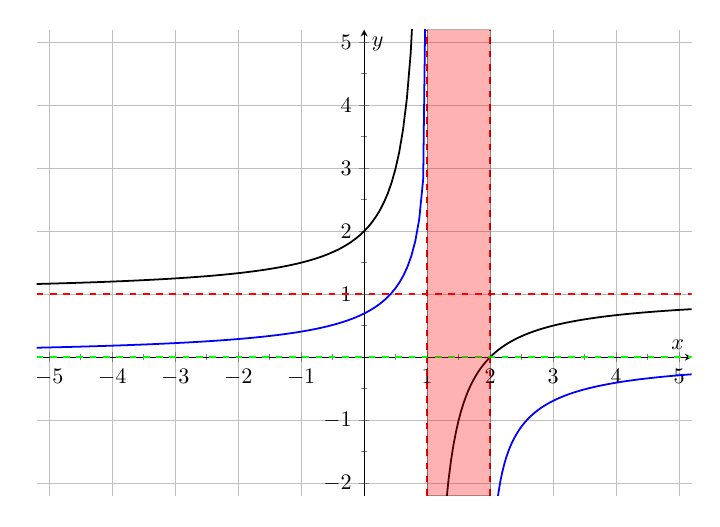
\begin{tikzpicture}[scale=0.8]
                \begin{axis}[
                    x=1.0cm,y=1.0cm,
                    axis lines=middle,
                    ymajorgrids=true,
                    xmajorgrids=true,
                    %xminorgrids=true,
                    %yminorgrids=true,
                    minor tick num=1,
                    xlabel = $x$,
                    ylabel =$y$,
                    xmin=-5.2,
                    xmax=5.2,
                    ymin=-2.2,
                    ymax=5.2,
                    xtick={-5.0,-4.0,...,5.0},
                    ytick={-2.0,-1.0,...,5.0},]
                    \draw [samples=100, domain=-5.2:0.8, thick] plot(\x,{(\x-2)/(\x-1)});
                    \draw [samples=100, domain=1.3:5.2, thick] plot(\x,{(\x-2)/(\x-1)});
                    \draw [dashed, color=red, thick] (-5.2,1)--(5.2,1);
                    \draw [dashed, color=red, thick] (1,-2.2)--(1,5.2);
                    \draw [dashed, color=red, thick] (2,-2.2)--(2,5.2);

                    \draw [dashed, color=green, thick] (-5.2,0)--(5.2,0);

                    \draw[fill=red, opacity=0.3] (1,-2.2)--(1,5.2)--(2,5.2)--(2,-2.2)--cycle;

                    %\draw [->] (-3.5,0.4)--(-4,0.4);
                    %\draw [->] (-1.3,3.5)--(-1.3,4);
                    %\draw [->] (-0.6,-2.4)--(-0.6,-2.9);
                    %\draw [->] (0.6,-2.4)--(0.6,-2.9);
                    %\draw [->] (1.3,3.5)--(1.3,4);
                    %\draw [->] (3.5,0.4)--(4,0.4);

                    \draw [samples=100, domain=-5.2:1, thick, color=blue] plot(\x,{ln((\x-2)/(\x-1))});
                    \draw [samples=100, domain=2.1:5.2, thick, color=blue] plot(\x,{ln((\x-2)/(\x-1))});
                    
                \end{axis}
            \end{tikzpicture}
        \end{figure} 
\newpage
\section{Studio di funzione completo}
    \subsection{Classificazione}
    \begin{tabular}{|c|c|c|c|}
        \hline
        \multirow{2}{4em}{Funzione} & algebrica\ & razionale & intera\\ \cline{2-4}
         & trascendente & irrazionale & fratta \\ \hline
    \end{tabular}
    \subsection{Dominio}
    \begin{itemize}
        \item Polinomiale : $\R$
        \item Fratte: denominatore $\neq 0$
        \item Irrazionali pari: radicando$\geq0$
        \item Irrazionali dispari: $\R$
        \item Logaritmi: argomento$>0$
        \item Esponenziali: $\R$
        \item Seno, coseno, arcotangente, arcocotangente: $\R$
        \item Tangente: $\R -{\frac{\pi}{2}+k\pi}\text{, con } k\in\Z$
        \item Cotangente: $\R -{k\pi}\text{, con } k\in\Z$
        \item Arcoseno, arcocoseno: $[-1;1]$
    \end{itemize}
    \subsection{Simmetrie}
    \textbf{CN:} $\forall x \in D, -x \in D$
    \begin{itemize}
        \item pari se $f(-x)=f(x)$
        \item dispari se $f(-x)=-f(x)$
    \end{itemize}
    \subsection{Intersezioni con gli assi cartesiani}
    \[f(x) \cap \text{asse~}x : \left\{\begin{array}{l}
         y=f(x)  \\
         y=0 
    \end{array}\right.~~~~~~~~ 
    f(x) \cap \text{asse~}y : \left\{\begin{array}{l}
         y=f(x)  \\
         x=0 
    \end{array}\right.\] 
    \subsection{Studio del segno}
    Risolvere la disequazione $f(x)>0$
    \subsection{Limiti, asintoti e discontinuità}
    \begin{tabular}{|m{0.3\textwidth}|m{0.6\textwidth}|}
        \hline
        Asintoto verticale&  \[\lim_{x\rightarrow x_0} f(x) = \infty\] \\\hline
        Asintoto orizzontale & \[\lim_{x\rightarrow \infty} f(x) = l\]\\ \hline
        Asintoto obliquo & \[\textnormal{CN: }\lim_{x\rightarrow\infty}f(x) = \infty\]
        \[m=\lim_{x\rightarrow\infty}\frac{f(x)}{x}\]
        \[q=\lim_{x\rightarrow\infty}f(x)-mx\] \\ \hline
    \end{tabular}\\
    \\
    \textbf{NB.:} Una funzione può avere anche infiniti asintoti verticali, ma al massimo due tra asintoti orizzontali e asintoti obliqui (uno destro e uno sinistro).\\    \begin{tabular}{|m{0.3\textwidth}|m{0.6\textwidth}|}
        \hline
        Prima specie &  \[\lim_{x\rightarrow x_0^-}f(x)=l_1~~~~\lim_{x\rightarrow x_0^+}f(x)=l_2\] \[l_1\neq l_2~~~~salto=|l_1-l_2|\]\\ \hline
        Seconda specie &  \[\lim_{x\rightarrow x_0^\pm}f(x)=\infty ~~~~\lor~~~~ \lim_{x\rightarrow x_0^\pm}f(x)=\nexists\] \\\hline
        Terza specie & \[\lim_{x\rightarrow x_0^-}f(x)=\lim_{x\rightarrow x_0^+}f(x)=l\]\[f(x_0)\neq l ~~~~ \lor ~~~~ f(x_0)=\nexists\]\\ \hline
    \end{tabular}
    \subsection{Derivata prima}
    Le soluzioni dell'equazione \[f'(x) = 0\] identificano la presenza di \begin{itemize}
        \item massimi relativi
        \item minimi relativi
        \item flessi a tangente orizzontale
    \end{itemize}
    Per distinguerli è necessario studiare il segno della derivata:
    \begin{figure}[h!]
        \centering
        \begin{subfigure}{0.48\textwidth}
            \centering
            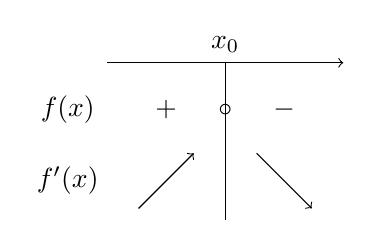
\begin{tikzpicture}
                \draw[->](0,0)--(3,0);
                \draw(1.5,0) node[above]{$x_0$}--(1.5,-2);
                \node at (-0.50, -0.60){$f(x)$};
                \node at (-0.50, -1.50){$f'(x)$};
                \node at (0.75,-0.60) {$+$};
                \node at (2.25,-0.60) {$-$};
                \node at (1.5, -0.60) {$\circ$};
                \draw[->] (0.4,-1.85)--(1.1,-1.15); %+ sx
                \draw[->] (1.9,-1.15)--(2.6,-1.85); %- dx
            \end{tikzpicture}
            \caption{Massimo relativo}
        \end{subfigure}
        \begin{subfigure}{0.48\textwidth}
            \centering
            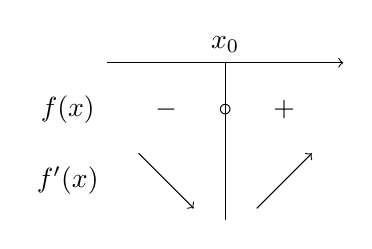
\begin{tikzpicture}
                \draw[->](0,0)--(3,0);
                \draw(1.5,0) node[above]{$x_0$}--(1.5,-2);
                \node at (-0.50, -0.60){$f(x)$};
                \node at (-0.50, -1.50){$f'(x)$};
                \node at (0.75,-0.60) {$-$};
                \node at (2.25,-0.60) {$+$};
                \node at (1.5, -0.60) {$\circ$};
                \draw[->] (0.4,-1.15)--(1.1,-1.85); %- sx
                \draw[->] (1.9,-1.85)--(2.6,-1.15); %+ dx
            \end{tikzpicture}
            \caption{Minimo relativo}
        \end{subfigure}
        \begin{subfigure}{0.48\textwidth}
            \centering
            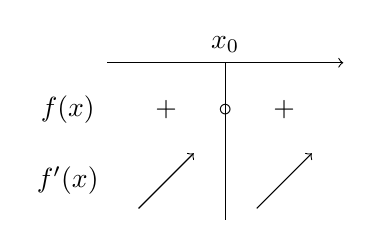
\begin{tikzpicture}
                \draw[->](0,0)--(3,0);
                \draw(1.5,0) node[above]{$x_0$}--(1.5,-2);
                \node at (-0.50, -0.60){$f(x)$};
                \node at (-0.50, -1.50){$f'(x)$};
                \node at (0.75,-0.60) {$+$};
                \node at (2.25,-0.60) {$+$};
                \node at (1.5, -0.60) {$\circ$};
                %\draw[->] (0.4,-1.15)--(1.1,-1.85); %- sx
                \draw[->] (0.4,-1.85)--(1.1,-1.15); %+ sx
                %\draw[->] (1.9,-1.15)--(2.6,-1.85); %- dx
                \draw[->] (1.9,-1.85)--(2.6,-1.15); %+ dx
            \end{tikzpicture}
            \caption{Flesso a tangente orizzontale ascendente}
        \end{subfigure}
        \begin{subfigure}{0.48\textwidth}
            \centering
            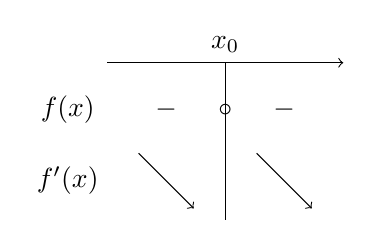
\begin{tikzpicture}
                \draw[->](0,0)--(3,0);
                \draw(1.5,0) node[above]{$x_0$}--(1.5,-2);
                \node at (-0.50, -0.60){$f(x)$};
                \node at (-0.50, -1.50){$f'(x)$};
                \node at (0.75,-0.60) {$-$};
                \node at (2.25,-0.60) {$-$};
                \node at (1.5, -0.60) {$\circ$};
                \draw[->] (0.4,-1.15)--(1.1,-1.85); %- sx
                \draw[->] (1.9,-1.15)--(2.6,-1.85); %- dx
            \end{tikzpicture}
            \caption{Flesso a tangente orizzontale discendente}
        \end{subfigure}
    \end{figure}
    Lo studio della derivata prima fornisce anche informazioni circa la monotonia della funzione.
    \subsection{Derivata seconda}
    Le soluzioni dell'equazione \[f''(x)=0\] permettono di identificare i punti di flesso. A differenza della derivata prima permette di ottenere informazioni circa la presenza di flessi a tangente obliqua, per cui è necessario escludere tutte le soluzioni già analizzate in precedenza. 
    La derivata seconda fornisce inoltre informazioni circa la concavità della funzione: verso l'alto quando la derivata seconda è positiva e verso il basso quando la derivata seconda è negativa. La funzione inverte la propria concavità in corrispondenza dei punti di flesso.
\end{document}